\documentclass[12pt,a4paper,final,twoside,onecolumn,titlepage]{book}
\usepackage[utf8]{inputenc} %File encoding
\usepackage[T1]{fontenc} % Use EC fonts
\usepackage{ae} % Fonts for PDF files
\usepackage{textcomp} % Text-Companion-Symbols (e. g. \texteuro)
\usepackage[english]{babel} % Language selection
\usepackage{lmodern} % Latin Modern

\usepackage{pdfpages}

%New Section Added for Coding
\usepackage{amsmath}
\usepackage{algorithm2e}
\usepackage{amsfonts}
\usepackage{amssymb}
\usepackage{graphicx}
\usepackage{natbib}
\usepackage{listings}
\usepackage{color}
\usepackage{textcomp}
\usepackage{multirow}
\definecolor{listinggray}{gray}{0.9}
\definecolor{lbcolor}{rgb}{0.9,0.9,0.9}
\lstset{
	backgroundcolor=\color{white},
	tabsize=4,
	rulecolor=,
	language=csh,
        basicstyle=\scriptsize,
        upquote=true,
        aboveskip={1.5\baselineskip},
        columns=fixed,
        showstringspaces=false,
        extendedchars=true,
        breaklines=true,
        prebreak = \raisebox{0ex}[0ex][0ex]{\ensuremath{\hookleftarrow}},
        frame=single,
        showtabs=false,
        showspaces=false,
        showstringspaces=false,
        identifierstyle=\ttfamily,
        keywordstyle=\color[rgb]{0,0,1},
        commentstyle=\color[rgb]{0.133,0.545,0.133},
        stringstyle=\color[rgb]{0.627,0.126,0.941},
}

%End of New Section Added for Coding

\usepackage[english]{translator}
%Load the package
\usepackage[
nonumberlist, %do not show page numbers
acronym,      %generate acronym listing
toc,          %show listings as entries in table of contents
section]      %use section level for toc entries
{glossaries}

\usepackage{hyperref}

\usepackage[utf8]{inputenc}
\usepackage{amsmath}
\usepackage{amsfonts}
\usepackage{amssymb}
\usepackage{graphicx}
\usepackage{natbib}
\author{Haitham A. El-Ghareeb, Ph.D.}
\title{Associate Professor}
\begin{document}

\cleardoublepage
\phantomsection
\tableofcontents

\chapter{C\# and Webservices}
\section{Quick Tour of C\#}
\subsection{Introduction}
This chapter is not intended to be an extensive C\# course. We are presenting here the fundamentals needed to understand the rest of the code presented in the book. Obviously this book is primarily about Data Structures and Algorithms, but in several places we will explore some aspects of using IronPython with other .NET languages, the foremost being C\#. If you don’t know C\#, this chapter will give you a brief over- view of the core parts of the language. It should be enough to let you read the code examples in the book, although you’ll probably want more detail if you’re trying to write C\# code.
\subsection{Namespaces}
Namespaces are similar to other languages packages and modules. The classes in an assembly live in namespaces, which can be nested to provide a hierarchical structure. This structure is used to group together related classes to make them easier to find. Namespaces are specified in C\# like so:
\lstset{language=csh, tabsize=4}
\begin{lstlisting}
namespace DataStructures.Professor { 
	class Haitham { 
		... 
	}
}
\end{lstlisting}
Here we declare a namespace called \texttt{DataStructures.Professor}, which contains the \texttt{Haitham} class. Another major feature of namespaces is that they enable us to avoid name collisions: the fully qualified name of the class is \texttt{DataStructures.Professor.Haitham}, and we could happily use other \texttt{Haitham} classes in our project as long as they are in different namespaces.
\subsection{Classes}
Class declarations in C\# are structured like this:
\lstset{language=csh, tabsize=4}
 \begin{lstlisting}
public class Haitham: Professor, IBlogger, IMozillaReMo { 
	public string name; 
	public Haitham(string name) {
		this.name = name; // more fields and methods here
}
\end{lstlisting}
The access modifier public before the class keyword indicates that the class is accessible outside the current namespace. The names after the colon specify what this class inherits from. Haitham is a subclass of the Professor class, as well as the IBlogger and IMozillaReMo interfaces. C\# doesn’t allow multiple inheritance of classes, but implementing multiple interfaces is fine. If no parent class is specified in a class definition (or it inherits only from interfaces), the class inherits from \texttt{System.Object}. The body of the class can contain definitions of various kinds of members:
\begin{itemize}
\item Constructors 
\item Fields (like the name attribute in the previous snippet) 
\item Methods 
\item Properties 
\item Events 
\item Operators
\end{itemize}
Each of these members has access modifiers as well:
\begin{itemize}
\item private—Can be used only inside this class 
\item protected—Accessible from this class and any subclasses 
\item internal—Accessible from any class in the current assembly 
\item public—Available from any code
\end{itemize}
Classes can also contain other types (including classes, interfaces, structs, or dele- gates) as members.
As well as access modifiers, other modifiers can be applied to classes when they are defined:
\begin{itemize}
\item abstract—This declares that the class can be used only as a base class and can’t be instantiated. It might contain declarations of abstract methods (without any implementation) that subclasses must define when they are declared. (Abstract classes can still contain concrete implementations of some methods.)
\item static—This indicates that this class can’t be instantiated or used as a type (so it can’t be subclassed). Static classes are essentially containers for their members.
\item sealed—This prevents this class from being subclassed, for security or performance reasons. When the compiler sees a method call on a sealed class, it can generate a direct call to the method, rather than a virtual call.
\item partial—Partial classes are classes that are defined in more than one file. This can be useful if some code in a class is machine generated; the generated code can be kept in a separate file and regenerated without clobbering the custom code.
\end{itemize}
\subsection{Attributes}
Attributes are declarative information that can be attached to different elements of a program and examined at runtime using reflection. They can be applied to types, methods, and parameters, as well as other items. The .NET framework defines a number of attributes, such as SerializableAttribute, STAThreadAttribute, and FlagsAttribute, which control various aspects of how the code runs. You can also create new attributes (to be interpreted by your own code) by inheriting from System.Attribute.
The following code applies the SecretOverrideAttribute to the ProfessorHaitham.Teach method:
\lstset{language=csh, tabsize=4}
\begin{center}
 \begin{lstlisting}
class ProfessorHaitham { 
	//...
	[SecretOverride("...")] public void Teach(Subjects datastructures2012) {
	//...
	}
}
 \end{lstlisting}
\end{center}
\subsection{Interfaces}
An interface is a type that defines methods and properties with no behavior. Its purpose is to make a protocol explicit without imposing any other restrictions on the implementation. For example, the previous \texttt{ProfessorHaitham} class implements the IMozillaReMo interface:
\begin{lstlisting}
interface IMozillaReMo {
	IBrowser FavouriteBrowser {get; set;} 
	void Browse();
}
\end{lstlisting}
This means that \texttt{ProfessorHaitham} must provide a definition of the \texttt{FavouriteBrowser} property and the \texttt{Browse} method. Classes that implement multiple interfaces must provide definitions for all of the interfaces’ members. Interfaces can subclass other interfaces (and even inherit from multiple interfaces), which means that they include all of the members of their bases as well as the members they declare.
Ordinarily, a class that inherits from an interface can implement its members simply by defining them with the correct name, parameters, and return type. In some cases, you might not want the interface members to be part of your class’s interface (for example, if you have two different interfaces that clash). You can implement those members explicitly, so that they are available only when used through a reference to the interface:
\begin{lstlisting}
public class ExplicitlyDriveable: IMozillaReMo { 
	// member prefixed with interface name 
	public void IMozillaReMo.Browse() {
	// implementation here... 
	// other members
	}
}
\end{lstlisting}
Then code trying to use the \texttt{Browse} method on an ExplicitlyDriveable instance
must cast it to IMozillaReMo first.
\subsection{Enums}
Enumerations are collections of named constants, which look like this:
\begin{lstlisting}
enum CoursesITeach { 
	DataStructuresAndAlgorithms,
	SystemAnalysisAndDesign, 
	ResearchMethodologies, 
	DataBase
}
\end{lstlisting}
The enum values can be referred to in code using \texttt{CoursesITeach.DataStruct\\uresAndAlgorithms}. By default, enumerations inherit from int, but they can be declared (using the inheritance syntax) as any of the integral .NET types: sbyte, byte, short, ushort, int, uint, long, or ulong. Enums can be combined as flags with the bitwise-or operator (|) if you annotate them with the Flags attribute, in which case you should also specify the value of each member (by default, they’re assigned sequentially from 0). For example, if you wanted the \texttt{CoursesITeach} values to be combinable, you could define it as follows:
\begin{lstlisting}
[Flags] 
enum CoursesITeach {
	DataStructuresAndAlgorithms = 1, 
	SystemAnalysisAndDesign = 2, 
	ResearchMethodologies = 4, 
	DataBase = 8
}
\end{lstlisting}
\subsection{Struct}
Structs are data structures that are defined similarly to classes. The difference is that a struct is a value type rather than a reference type like a class. When a variable is of a class type, it contains a reference to an instance of the class (or null). A struct variable directly contains the members of the struct rather than being a reference to an object elsewhere in memory. This is generally useful for performance or memory optimization: a large array of structs can be much quicker to create than the same size array of objects. In some situations using structs can be slower, though, particularly when assigning or passing them as parameters (because all their member data needs to be copied). 
Struct definitions look like this:
\begin{lstlisting}
struct Faculty { 
	public float name; 
	public Faculty(String name) {
		//...
	}
}
\end{lstlisting}
Structs can’t inherit from any type (other than object, which they inherit from
implicitly), and no types can inherit from them.
\subsection{Methods}
Methods in C\# are members of classes and structs that are defined by giving the access level, the return type, the name of the method, and the parameters it accepts, as well as the block of code that is executed when it is called:
\begin{lstlisting}
class Haitham { 
	//...
	public void GoToLecture(string LectureName) { 
		Point location = this.targetDatabase.Find(targetName); 
		this.FlyToLocation(location);
	}
}
\end{lstlisting}
The void return type indicates that this method returns nothing.
\subsubsection{Virtual and override Methods}
The virtual modifier applied to a method indicates that it can be overridden in a subclass. The subclass’s version of the method must have the same visibility, name, parameter types, and return type as the base class method and be defined using the keyword override.
\begin{lstlisting}
class GiantRobot { 
	//...
	public virtual void TravelTo(Point destination) { 
		this.TurnTowards(destination); 
		while (this.Location != destination) {
			this.Trudge();
		}
	}
}

class FlyingRobot: GiantRobot { 
	//...
	public override void TravelTo(Point destination) { 
		if (this.WingState == WingState.Operational) {
			this.FlyTo(destination); 
			// whee! 
		} else {
			base.TravelTo(destination); // oh well...
		}	
	}
}
\end{lstlisting}
In a method, \texttt{this} refers to the current instance, although this doesn’t need to be a parameter of each method. To call a superclass method or property (for example, from the body of an override method), you refer to base. Semantics are simpler because any C\# class has only one superclass.
\subsubsection{Other method modifiers}
A number of other modifiers can be included after the access modifier when defining a method. The more commonly seen modifiers are these:
\begin{itemize}
\item static—This method must be called directly on the class rather than on an instance (and so can’t refer to this).
\item sealed—This override method can’t be overridden again in a subclass. This is often done for performance or security reasons.
\item abstract—This method must be implemented in subclasses. Abstract methods can’t contain any code.
\end{itemize}
\subsubsection{Parameter passing}
By default, method parameters are passed by object value (with the extra wrinkle that structs are copied).
In C\# you can change this behavior using the ref and out parameter modifiers. If a parameter has the ref modifier, it is passed by reference instead. Assignments to that parameter in the method will be reflected in the variable passed in by the caller. For example, an int variable passed as a ref parameter can be assigned in the method, and the variable’s value will be updated in the calling scope. Out parameters are similar, with the difference that they don’t need to be assigned a value before calling the method, and they must be assigned in the method. The difference between them is that out parameters are viewed as extra return values of the method, while ref parameters are values that are both input and potentially output of the method.
\subsection{Method overloading}
There can be multiple different methods in a class with the same name, as long as the combination of name and parameter types is unique within the class. Methods that have the same name but different parameters are said to be overloaded. When you call an overloaded method, the compiler uses the compile-time types of the parameters passed in to determine which version of the method is called. This is an important distinction between overload dispatch, where the selection of which overload to call is purely based on the declared types of the parameters, and method dispatch, where the method called is determined by the type of the instance at runtime, regardless of the declared type of the variable.
\subsection{Loops}
C\# has four looping constructs: while, do, for, and foreach.
\subsubsection{while loop}
The condition of the loop in C\# must evaluate to a bool.
\begin{lstlisting}
int a = 10; 
while (a > 0) {
	a--;
}
\end{lstlisting}
The loop control keywords break and continue work (for all C\# loops). The condition of the loop must be included in parentheses.
\subsubsection{do loop}
The do loop is like a while loop, where the condition is checked at the end of the loop body; that is, the loop body always executes at least once.
\begin{lstlisting}
int a = 0; 
do {
	a--; } while (a > 0);
\end{lstlisting}
After the execution of this loop, a will have the value -1.


\subsubsection{for loop}
The C\# for loop has three parts in addition to the loop body:
\begin{itemize}
\item An initialization clause, which sets up variables before the loop begins 
\item A condition that is tested before each execution of the loop body 
\item An iteration clause, which is executed after each execution of the loop body
\end{itemize}
Here’s an example:
\begin{lstlisting}
int total = 0; 
for (int i = 0; i < 10; i++) {
	total += i;
}
\end{lstlisting}
After execution, total will have the value 45 (the sum of 0 to 9), because it stops when i equals 1. Each of the three control clauses is optional, and each clause can consist of multiple statements separated by commas.


\subsubsection{foreach loop}
The foreach loop can iterate over any collection that implements the IEnumerable interface, including arrays.
\begin{lstlisting}
string[] names = new string[] {"Haitham", "Mohamed", "Hesham"}; 
foreach (string person in names} {
	Console.WriteLine(person);
}
\end{lstlisting}
\subsection{if}
The condition must be in parentheses and yield a Boolean. If statements can be chained, so there’s no need for the elif.
\begin{lstlisting}
if (!robot.AtDestination()) { 
	robot.Walk();
} else if (robot.CanSee(target)) { 
		robot.Destroy(target);
	} else { 
		robot.ChillOut();
}
\end{lstlisting}
\subsection{switch}
Some situations that would require an if-elif-else construct or a dictionary lookup can be done more cleanly in C\# using a switch statement.
\begin{lstlisting}
MaterialSelection file; 
switch (target.Type) {
	case TargetType.DataStructuresAndAlgorithms: 
		book = "Data Structures and Algorithms using C\# and Python"; 
		break;
	case TargetType.DataBase: 
		book = "Database Management Systems, Thomas Conolley"; 
		break;
	case TargetType.ImageProcessing: 
	case TargetType.OpenCV:
		book = "Open CV Reference Book";
		break; 
	case default:
		book = null; 
		break;
\end{lstlisting}
The case labels must be constants, and each case has to end with a flow-control statement like break, throw, or return; execution isn’t allowed to fall through from one case to another. If you want fall-through behavior, you can use the goto case statement to explicitly jump to the case that should be executed. Two case labels together (like the ImageProcessing and OpenCV case shown previously) are treated as if they share the same body. If the switch expression doesn’t match any of the case labels and there’s a default case, it is executed.
\subsection{try/catch/finally and throw}
\begin{lstlisting}
try { 
	robot.ReturnToBase(TransportMode.FootThrusters);
} catch (FootThrusterFailure) { 
	robot.ReturnToBase(TransportMode.BoringWalking);
} catch (EmergencyOverrideException e) { 
	robot.SelectTarget(e.NewTarget);
} catch { robot.AssumeDefensivePosition(); 
	throw; // re-throw the original exception
} finally { 
	robot.NotifyBase();
}
\end{lstlisting}
\subsection{null}
null, a value that is the singleton instance of NoneType. null is a reference that doesn’t refer to any object. This has two consequences: first, null can be assigned to a variable of any reference type, and second, value types like int, DateTime, or custom structs can’t be null, because they don’t contain references.
The second fact can be inconvenient in some situations, so each value type in C\# has a nullable version, represented with the type name followed by a question mark. For example, a nullable integer variable would be declared with int?. Nullable types can then be used as normal (although there are performance differences under the hood) and be assigned null in the same way as reference types.
\subsection{Excercises}
\textbf{Problem:}\\
If we list all the natural numbers below 10 that are multiples of 3 or 5, we get 3, 5, 6 and 9. The sum of these multiples is 23.
Find the sum of all the multiples of 3 or 5 below 1000.\\
\textbf{\textit{Hint:}} Answer: 233168\\
Thanks to http://projecteuler.net/problem=1
\textbf{Problem}
Write the Programs needed to solve the following problems:
\begin{itemize}
\item Program to compute $\sum_{i}^{n}=1^{i}$
\item Program to compute $\sum_{i}^{n}=1^{i}$ using Horner's rule.
\item Program to compute $\gamma$
\item Program to compute $\sum_{i}^{n}=x_{0}^{i}$
\item Program to compute $\sum_{i}^{n}=x_{0}^{i}$ using Horner's rule.
\item Program to compute $\sum_{i}^{n}=x_{0}^{i}$ using the closed-form expression.
\item Program to compute $\sum_{i=0}^{j}a_{i}$ for $0\leq j<n$
\item Program to compute $n!$
\end{itemize}




\newpage
%Print the glossary
\printglossary[style=altlist,title=Glossary]


\bibliographystyle{plain}

\chapter{Python and Webservices}
\section{Python Crash Course}
\subsection{Introduction}
Python is an easy to learn, powerful programming language. It has efficient high-level data structures and a simple but effective approach to object-oriented programming. Python’s elegant syntax and dynamic typing, together with its interpreted nature, make it an ideal language for scripting and rapid application development in many areas on most platforms. The Python interpreter and the extensive standard library are freely available in source or binary form for all major platforms from the Python Web site, http://www.python.org/, and may be freely distributed. The same site also contains distributions of and pointers to many free third party Python modules, programs and tools, and additional documentation.

The Python interpreter is easily extended with new functions and data types implemented in C or C++ (or other languages callable from C). Python is also suitable as an extension language for customizable applications. This chapter introduces you to the basic concepts and features of the Python language and system. It helps to have a Python interpreter handy for hands-on experience, but all examples are self-contained, so the tutorial can be read off-line as well.

For a description of standard objects and modules, see The Python Standard Library. The Python Language Reference gives a more formal definition of the language. To write extensions in C or C++, read Extending and Embedding the Python Interpreter and Python/C API Reference Manual. There are also several books covering Python in depth. This chapter does not attempt to be comprehensive and cover every single feature, or even every commonly used feature. Instead, it introduces many of Python’s most noteworthy features, and will give you a good idea of the language’s flavor and style. After reading it, you will be able to read and write Python modules and programs, and you will be ready to learn more about the various Python library modules described in The Python Standard Library.

\subsection{Compilers vs. Interpreters}
In Programming Languages, we write statements like:\\
\texttt{c = a + b}\\
This needs to be translated into machine language that the computer can execute. Compilers convert programs written in a high-level language into the machine language of some computer. Interpreters simulate a computer that understands a high-level language. In Interpreted languages, the source program is not translated into machine language all at once. An interpreter analyzes and executes the source code instruction by instruction. In Compiled languages, once program is compiled, it can be executed over and over without the source code or compiler. If it is interpreted, the source code and interpreter are needed each time the program runs. Compiled programs generally run faster since the translation of the source code happens only once. Interpreted languages are part of a more flexible programming environment since they can be developed and run interactively
Interpreted programs are more portable, meaning the executable code produced from a compiler for a Pentium won’t run on a Mac, without recompiling. If a suitable interpreter already exists, the interpreted code can be run with no modifications.

\subsection{Python Magic}
When you start Python, you will see something like:
\lstset{language=Python, tabsize=4}
\begin{lstlisting}
Python 3.1.2 (r312:79149, Mar 21 2010, 00:41:52) [MSC v.1500 32 bit (Intel)] on win32
Type "copyright", "credits" or "license()" for more information.
>>> 
\end{lstlisting}
The $>>>$ is a Python prompt indicating that Python is ready for us to give it a command. These commands are called statements.
\lstset{language=Python, tabsize=4}
\begin{lstlisting}
>>> print("Hello Haitham!")
Hello Haitham
>>> print (5+4)
9
>>> print("5+4=",5+4)
5+4=9
>>>
\end{lstlisting}
Usually we want to execute several statements together that solve a common problem. One way to do this is to use a function.
\lstset{language=Python, tabsize=4}
\begin{lstlisting}
>>> def hello():
	    print("Hello") 
	    print("Computers are Fun") 
	    	
>>> 
The Magic of Python
>>> def hello():
	    print("Hello") 
	    print("Computers are Fun") 

>>>
\end{lstlisting}
The first line tells Python we are defining a new function called hello. The following lines are indented to show that they are part of the hello function. The blank line (hit enter twice) lets Python know the definition is finished.
\lstset{language=Python, tabsize=4}
\begin{lstlisting}
>>> def hello():
	   print("Hello")
	   print("Computers are Fun") 
	
>>>
\end{lstlisting}
Notice that nothing has happened yet! We’ve defined the function, but we haven’t told Python to perform the function! A function is invoked by typing its name.
\lstset{language=Python, tabsize=4}
\begin{lstlisting}
>>> hello()
Hello
Computers are Fun
>>> 
\end{lstlisting}
Commands can have changeable parts called parameters that are placed between the ()’s.
\lstset{language=Python, tabsize=4}
\begin{lstlisting}
>>> def greet(person):
	    print("Hello",person)
	    print ("How are you?")
	
>>> 

>>> greet("Haitham")
Hello Haitham
How are you?
>>> greet("Sakr")
Hello Sakr
How are you?
>>>  
\end{lstlisting}
When we use parameters, we can customize the output of our function. When we exit the Python prompt, the functions we’ve defined cease to exist! Programs are usually composed of functions, modules, or scripts that are saved on disk so that they can be used again and again. A module file is a text file created in text editing software (saved as “plain text”) that contains function definitions. A programming environment is designed to help programmers write programs and usually includes automatic indenting, highlighting, etc.

\lstset{language=Python, tabsize=4}
\begin{lstlisting}
# File: chaos.py
# A simple program illustrating chaotic behavior

def main():
    print("This program illustrates a chaotic function")
    x = eval(input("Enter a number between 0 and 1: "))
    for i in range(10):
        x = 3.9 * x * (1 - x)
        print(x)

main()
\end{lstlisting}
We’ll use filename.py when we save our work to indicate it’s a Python program. In this code we’re defining a new function called main. The main() at the end tells Python to run the code.
\lstset{language=Python, tabsize=4}
\begin{lstlisting}
>>> 
This program illustrates a chaotic function
Enter a number between 0 and 1: .5
0.975
0.0950625
0.335499922266
0.869464925259
0.442633109113
0.962165255337
0.141972779362
0.4750843862
0.972578927537
0.104009713267
>>> 
\end{lstlisting}
\subsection{Temprature Converter}
Example Program: Temperature Converter
\lstset{language=Python, tabsize=4}
\begin{lstlisting}
#convert.py
# A program to convert Celsius temps to Fahrenheit
# by: Susan Computewell

def main():
    celsius = eval(input("What is the Celsius temperature? "))
    fahrenheit = (9/5) * celsius + 32
    print("The temperature is ",fahrenheit," degrees Fahrenheit.")

main()
\end{lstlisting}
Once we write a program, we should test it!
\lstset{language=Python, tabsize=4}
\begin{lstlisting}
>>> 
What is the Celsius temperature? 0
The temperature is  32.0  degrees Fahrenheit.
>>> main()
What is the Celsius temperature? 100
The temperature is  212.0  degrees Fahrenheit.
>>> main()
What is the Celsius temperature? -40
The temperature is  -40.0  degrees Fahrenheit.
>>> 
\end{lstlisting}
\subsection{Elements of Programs}
\subsubsection{Names}
Names are given to variables (celsius, fahrenheit), modules (main, convert), etc. These names are called identifiers Every identifier must begin with a letter or underscore, followed by any sequence of letters, digits, or underscores. Identifiers are case sensitive. These are all different, valid names:
\begin{itemize}
\item X
\item Celsius
\item Spam
\item spam
\item spAm
\item Spam\_ and\_ Eggs
\item Spam\_ And\_ Eggs
\end{itemize}
Some identifiers are part of Python itself. These identifiers are known as reserved words. This means they are not available for you to use as a name for a variable, etc. in your program. Python reserved words include:
\begin{itemize}
\item and 
\item del
\item for
\item is
\item raise
\item assert
\item elif
\item in
\item print
\end{itemize}
\subsubsection{Expressions}
The fragments of code that produce or calculate new data values are called expressions. Literals are used to represent a specific value, e.g. 3.9, 1, 1.0. Simple identifiers can also be expressions.
\lstset{language=Python, tabsize=4}
\begin{lstlisting}
>>> x = 5
>>> x
5
>>> print(x)
5
>>> print(spam)

Traceback (most recent call last):
  File "<pyshell#15>", line 1, in -toplevel-
    print spam
NameError: name 'spam' is not defined
>>> 
\end{lstlisting}
NameError is the error when you try to use a variable without a value assigned to it. Simpler expressions can be combined using operators. +, -, *, /, ** . Spaces are irrelevant within an expression. The normal mathematical precedence applies.
((x1 – x2) / 2*n) + (spam / k**3)
\subsubsection{Output Statements}
A print statement can print any number of expressions. Successive print statements will display on separate lines. A bare print will print a blank line.
\lstset{language=Python, tabsize=4}
\begin{lstlisting}
print(3+4)
print(3, 4, 3+4)
print()
print(3, 4, end=" "),
print(3 + 4)
print("The answer is", 3+4)
7
3 4 7

3 4 7
The answer is 7
\end{lstlisting}

\subsubsection{Assignment Statements}
Simple Assignment
<variable> = <expr>
variable is an identifier, expr is an expression
The expression on the RHS is evaluated to produce a value which is then associated with the variable named on the LHS.
x = 3.9 * x * (1-x)
fahrenheit = 9/5 * celsius + 32
x = 5
Variables can be reassigned as many times as you want!
\lstset{language=Python, tabsize=4}
\begin{lstlisting}
>>> myVar = 0
>>> myVar
0
>>> myVar = 7
>>> myVar
7
>>> myVar = myVar + 1
>>> myVar
8
>>> 
\end{lstlisting}
Variables are like a box we can put values in. When a variable changes, the old value is erased and a new one is written in. Technically, this model of assignment is simplistic for Python. Python doesn't overwrite these memory locations (boxes). Assigning a variable is more like putting a “sticky note” on a value and saying, “this is x”.
\subsubsection{Assigning Input}
The purpose of an input statement is to get input from the user and store it into a variable.
<variable> = eval(input(<prompt>))
First the prompt is printed The input part waits for the user to enter a value and press <enter>. The expression that was entered is evaluated to turn it from a string of characters into a Python value (a number). The value is assigned to the variable.
\subsubsection{Simultaneous Assignment}
Several values can be calculated at the same time
<var>, <var>, … = <expr>, <expr>, …
Evaluate the expressions in the RHS and assign them to the variables on the LHS
sum, diff = x+y, x-y
\subsubsection{Swapping Using Simultaneous Assignment}
We can swap the values of two variables quite easily in Python!
\lstset{language=Python, tabsize=4}
\begin{lstlisting}
x, y = y, x
>>> x = 3
>>> y = 4
>>> print x, y
3 4
>>> x, y = y, x
>>> print x, y
4 3
\end{lstlisting}
We can use this same idea to input multiple variables from a single input statement!
\subsubsection{Use commas to separate the inputs}
\lstset{language=Python, tabsize=4}
\begin{lstlisting}
def spamneggs():
	spam, eggs = eval(input("Enter # of slices of spam followed by # of eggs: "))
	print ("You ordered", eggs, "eggs and", spam, "slices of spam.")
	
>>> spamneggs()
Enter the number of slices of spam follwed by the number of eggs: 3, 2
You ordered 2 eggs and 3 slices of spam.
\end{lstlisting}

\subsubsection{Definite Loops}
A definite loop executes a definite number of times, i.e., at the time Python starts the loop it knows exactly how many iterations to do.
for <var> in <sequence>:
	<body>
The beginning and end of the body are indicated by indentation.
Definite Loops
for <var> in <sequence>:
<body>
The variable after the for is called the loop index. It takes on each successive value in sequence.
\lstset{language=Python, tabsize=4}
\begin{lstlisting}
>>> for i in [0,1,2,3]:
	print (i)

0
1
2
3
>>> for odd in [1, 3, 5, 7]:
	print(odd*odd)

1
9
25
49

>>> 
\end{lstlisting}
In chaos.py, what did range(10) do?
\lstset{language=Python, tabsize=4}
\begin{lstlisting}
>>> list(range(10))
[0, 1, 2, 3, 4, 5, 6, 7, 8, 9]
\end{lstlisting}
range is a built-in Python function that generates a sequence of numbers, starting with 0. list is a built-in Python function that turns the sequence into an explicit list. The body of the loop executes 10 times. for loops alter the flow of program execution, so they are referred to as control structures.

\subsection{Numeric Data Types}
The information that is stored and manipulated bu computers programs is referred to as data. There are two different kinds of numbers!
\\(5, 4, 3, 6) are whole numbers – they don’t have a fractional part
\\(.25, .10, .05, .01) are decimal fractions
Inside the computer, whole numbers and decimal fractions are represented quite differently! We say that decimal fractions and whole numbers are two different data types. The data type of an object determines what values it can have and what operations can be performed on it. Whole numbers are represented using the integer (int for short) data type. These values can be positive or negative whole numbers. Numbers that can have fractional parts are represented as floating point (or float) values.
How can we tell which is which?
\begin{itemize}
\item A numeric literal without a decimal point produces an int value
\item A literal that has a decimal point is represented by a float (even if the fractional part is 0)
\end{itemize}
Python has a special function to tell us the data type of any value.
\lstset{language=Python, tabsize=4}
\begin{lstlisting}
>>> type(3)
<class 'int'>
>>> type(3.1)
<class 'float'>
>>> type(3.0)
<class 'float'>
>>> myInt = 32
>>> type(myInt)
<class 'int'>
>>> 
\end{lstlisting}
\subsubsection{Why do we need two number types?}
Values that represent counts can’t be fractional (you can’t have 3 ½ quarters). Most mathematical algorithms are very efficient with integers. The float type stores only an approximation to the real number being represented! Since floats aren’t exact, use an int whenever possible! Operations on ints produce ints, operations on floats produce floats (except for /).
\lstset{language=Python, tabsize=4}
\begin{lstlisting}
>>> 3.0+4.0
7.0
>>> 3+4
7
>>> 3.0*4.0
12.0
>>> 3*4
12
>>> 10.0/3.0
3.3333333333333335
>>> 10/3
3.3333333333333335
>>> 10 // 3
3
>>> 10.0 // 3.0
3.0
\end{lstlisting}
Integer division produces a whole number. That’s why 10//3 = 3!
Think of it as ‘gozinta’, where 10//3 = 3 since 3 gozinta (goes into) 10 3 times (with a remainder of 1)
10\%3 = 1 is the remainder of the integer division of 10 by 3.
\\a = (a/b)(b) + (a\%b)
\subsection{Using the Math Library}
Besides (+, -, *, /, //, **, \%, abs), we have lots of other math functions available in a math library. A library is a module with some useful definitions/functions.  To use a library, we need to make sure this line is in our program:
\lstset{language=Python, tabsize=4}
\begin{lstlisting}
import math
\end{lstlisting}
Importing a library makes whatever functions are defined within it available to the program. To access the sqrt library routine, we need to access it as math.sqrt(x). Using this dot notation tells Python to use the sqrt function found in the math library module.
To calculate the root, you can do:
discRoot = math.sqrt(b*b – 4*a*c)
\lstset{language=Python, tabsize=4}
\begin{lstlisting}
# quadratic.py
#    A program that computes the real roots of a quadratic equation.
#    Illustrates use of the math library.
#    Note: This program crashes if the equation has no real roots.

import math  # Makes the math library available.

def main():
    print("This program finds the real solutions to a quadratic")
    print()

    a, b, c = eval(input("Please enter the coefficients (a, b, c): "))

    discRoot = math.sqrt(b * b - 4 * a * c)
    root1 = (-b + discRoot) / (2 * a)
    root2 = (-b - discRoot) / (2 * a)

    print()
    print("The solutions are:", root1, root2 )

main()
\end{lstlisting}

\subsection{Accumulating Results: Factorial}
Say you are waiting in a line with five other people. How many ways are there to arrange the six people?
720 -- 720 is the factorial of 6 (abbreviated 6!)
Factorial is defined as:
n! = n(n-1)(n-2)…(1)
So, 6! = 6*5*4*3*2*1 = 720
How we could we write a program to do this?
\begin{itemize}
\item Input number to take factorial of, n
\item Compute factorial of n, fact
\item Output fact
\end{itemize}
How did we calculate 6!?
\begin{enumerate}
\item 6*5 = 30
\item Take that 30, and 30 * 4 = 120
\item Take that 120, and 120 * 3 = 360
\item Take that 360, and 360 * 2 = 720
\item Take that 720, and 720 * 1 = 720
\end{enumerate}
We’re doing repeated multiplications, and we’re keeping track of the running product. This algorithm is known as an accumulator, because we’re building up or accumulating the answer in a variable, known as the accumulator variable.
The general form of an accumulator algorithm looks like this:
\begin{itemize}
\item Initialize the accumulator variable
\item Loop until final result is reached
\item update the value of accumulator variable
\end{itemize}
It looks like we’ll need a loop!
\lstset{language=Python, tabsize=4}
\begin{lstlisting}
fact = 1
for factor in [6, 5, 4, 3, 2, 1]:
	fact = fact * factor
\end{lstlisting}
Why did we need to initialize fact to 1? Because: Each time through the loop, the previous value of fact is used to calculate the next value of fact. By doing the initialization, you know fact will have a value the first time through. Since multiplication is associative and commutative, we can rewrite our program as:
\lstset{language=Python, tabsize=4}
\begin{lstlisting}
fact = 1
for factor in [2, 3, 4, 5, 6]:
	fact = fact * factor
\end{lstlisting}
We use range(n):
0, 1, 2, 3, …, n-1
range has another optional parameter! range(start, n) returns
start, start + 1, …, n-1
range(start, n, step)
start, start+step, …, n-1
list(<sequence>) to make a list
\lstset{language=Python, tabsize=4}
\begin{lstlisting}
>>> list(range(10))
[0, 1, 2, 3, 4, 5, 6, 7, 8, 9]
>>> list(range(5,10))
[5, 6, 7, 8, 9]
>>> list(range(5,10,2))
[5, 7, 9]
\end{lstlisting}
We can count up from 2 to n:
range(2, n+1)
(Why did we have to use n+1?)
We can count down from n to 2:
range(n, 1, -1)
Our completed factorial program:
\lstset{language=Python, tabsize=4}
\begin{lstlisting}
# factorial.py
#    Program to compute the factorial of a number
#    Illustrates for loop with an accumulator

def main():
    n = eval(input("Please enter a whole number: "))
    fact = 1
    for factor in range(n,1,-1): 
       fact = fact * factor
    print("The factorial of", n, "is", fact)

main()
\end{lstlisting}
\subsection{The Limits of Int}
What is 100!?
\lstset{language=Python, tabsize=4}
\begin{lstlisting}
>>> main()
Please enter a whole number: 100
The factorial of 100 is 93326215443944152681699238856266700490715968264381621468592963895217599993229915608941463976156518286253697920827223758251185210916864000000000000000000000000
\end{lstlisting}
Newer versions of Python can handle it, but…
\lstset{language=Python, tabsize=4}
\begin{lstlisting}
Python 1.5.2 (#0, Apr 13 1999, 10:51:12) [MSC 32 bit (Intel)] on win32
Copyright 1991-1995 Stichting Mathematisch Centrum, Amsterdam
>>> import fact
>>> fact.main()
Please enter a whole number: 13
13
12
11
10
9
8
7
6
5
4
Traceback (innermost last):
  File "<pyshell#1>", line 1, in ?
    fact.main()
  File "C:\PROGRA~1\PYTHON~1.2\fact.py", line 5, in main
    fact=fact*factor
OverflowError: integer multiplication
\end{lstlisting}
While there are an infinite number of integers, there is a finite range of ints that can be represented. This range depends on the number of bits a particular CPU uses to represent an integer value. Typical PCs use 32 bits. Typical PCs use 32 bits. That means there are 232 possible values, centered at 0. This range then is –231 to 231-1. We need to subtract one from the top end to account for 0. But our 100! is much larger than this. How does it work?
\subsubsection{Handling Large Numbers}
Does switching to float data types get us around the limitations of ints?
If we initialize the accumulator to 1.0, we get
\lstset{language=Python, tabsize=4}
\begin{lstlisting}
>>> main()
Please enter a whole number: 15
The factorial of 15 is 1.307674368e+012
\end{lstlisting}
We no longer get an exact answer!
\subsubsection{Long Int}
Very large and very small numbers are expressed in scientific or exponential notation.
1.307674368e+012 means 1.307674368 * 1012
Here the decimal needs to be moved right 12 decimal places to get the original number, but there are only 9 digits, so 3 digits of precision have been lost.
\subsubsection{Floats are approximations}
Floats allow us to represent a larger range of values, but with lower precision. Python has a solution, expanding ints! Python Ints are not a fixed size and expand to handle whatever value it holds. Newer versions of Python automatically convert your ints to expanded form when they grow so large as to overflow. We get indefinitely large values (e.g. 100!) at the cost of speed and memory
\subsection{Type Conversions}
We know that combining an int with an int produces an int, and combining a float with a float produces a float. What happens when you mix an int and float in an expression?
x = 5.0 + 2
For Python to evaluate this expression, it must either convert 5.0 to 5 and do an integer addition, or convert 2 to 2.0 and do a floating point addition. Converting a float to an int will lose information. Ints can be converted to floats by adding “.0”. In mixed-typed expressions Python will convert ints to floats. Sometimes we want to control the type conversion. This is called explicit typing.
\lstset{language=Python, tabsize=4}
\begin{lstlisting}
>>> float(22//5)
4.0
>>> int(4.5)
4
>>> int(3.9)
3
>>> round(3.9)
4
>>> round(3)
3
\end{lstlisting}

\subsection{Object Oriented Programming}
Each data type can represent a certain set of values, and each had a set of associated operations. The traditional programming view is that data is passive – it’s manipulated and combined with active operations. Modern computer programs are built using an object-oriented approach. Most applications you’re familiar with have Graphical User Interfaces (GUI) that provide windows, icons, buttons and menus. Basic idea – view a complex system as the interaction of simpler objects. An object is a sort of active data type that combines data and operations. Objects know stuff (contain data) and they can do stuff (have operations). Objects interact by sending each other messages.
Suppose we want to develop a data processing system for a college or university. We must keep records on students who attend the school. Each student will be represented as an object. The student object would contain data like:
\begin{itemize}
\item Name
\item ID number
\item Courses taken
\item Campus Address
\item Home Address
\item GPA
\end{itemize}
The student object should also respond to requests. We may want to send out a campus-wide mailing, so we’d need a campus address for each student. We could send the printCampusAddress to each student object. When the student object receives the message, it prints its own address. Objects may refer to other objects. Each course might be represented by an object:
\begin{itemize}
\item Instructor
\item Student roster
\item Prerequisite courses
\item When and where the class meets
\end{itemize}
Sample Operations:
\begin{itemize}
\item addStudent
\item delStudent
\item changeRoom
\end{itemize}
Computation is preformed by asking an object to carry out one of its operations. Each object is an instance of some class, and the class describes the properties of the instance.  To create a new instance of a class, we use a special operation called a constructor.
<class-name>(<param1>, <param2>, …)
<class-name> is the name of the class we want to create a new instance of, e.g. Circle or Point.
The parameters are required to initialize the object. For example, Point requires two numeric values.
p = Point(50, 60)
The constructor for the Point class requires to parameters, the x and y coordinates for the point.
These values are stored as instance variables inside of the object.
To perform an operation on an object, we send the object a message. The set of messages an object responds to are called the methods of the object. Methods are like functions that live inside the object.
Methods are invoked using dot-notation:
<object>.<method-name>(<param1>, <param2>, …)
p.getX() and p.getY() returns the x and y values of the point. Routines like these are referred to as accessors because they allow us to access information from the instance variables of the object.
Other methods change the state of the object by changing the values of the object’s instance variables.
move(dx, dy) moves the object dx units in the x direction and dy in the y direction.
Move erases the old image and draws it in its new position. Methods that change the state of an object are called mutators.
It’s possible for two different variables to refer to the same object – changes made to the object through one variable will be visible to the other.
\begin{lstlisting}
>>> leftEye = Circle(Point(80,50), 5)
>>> leftEye.setFill('yellow')
>>> leftEye.setOutline('red')
>>> rightEye = leftEye
>>> rightEye.move(20,0)
\end{lstlisting}
The idea is to create the left eye and copy that to the right eye which gets moved 20 units. The assignment rightEye = leftEye makes rightEye and leftEye refer to the same circle! The situation where two variables refer to the same object is called aliasing.

\subsection {Interactive Graphics}
In a GUI environment, users typically interact with their applications by clicking on buttons, choosing items from menus, and typing information into on-screen text boxes.
Event-driven programming draws interface elements (widgets) on the screen and then waits for the user to do something. An event is generated whenever a user moves the mouse, clicks the mouse, or types a key on the keyboard.
An event is an object that encapsulates information about what just happened! The event object is sent to the appropriate part of the program to be processed, for example, a button event.

\subsection{The String Data Type}
The most common use of personal computers is word processing. Text is represented in programs by the string data type.
A string is a sequence of characters enclosed within quotation marks (") or apostrophes (').
\begin{lstlisting}
>>> str1="Hello"
>>> str2='spam'
>>> print(str1, str2)
Hello spam
>>> type(str1)
<class 'str'>
>>> type(str2)
<class 'str'>
\end{lstlisting}

\subsubsection{Getting a string as input}
\begin{lstlisting}
>>> firstName = input("Please enter your name: ")
Please enter your name: John
>>> print("Hello", firstName)
Hello John
\end{lstlisting}
Notice that the input is not evaluated. We want to store the typed characters, not to evaluate them as a Python expression. We can access the individual characters in a string through indexing. The positions in a string are numbered from the left, starting with 0. The general form is <string>[<expr>], where the value of expr determines which character is selected from the string.
\begin{lstlisting}
>>> greet = "Hello Bob"
>>> greet[0]
'H'
>>> print(greet[0], greet[2], greet[4])
H l o
>>> x = 8
>>> print(greet[x - 2])
B
\end{lstlisting}
In a string of n characters, the last character is at position n-1 since we start counting with 0. We can index from the right side using negative indexes.
\begin{lstlisting}
>>> greet[-1]
'b'
>>> greet[-3]
'B'
\end{lstlisting}
Indexing returns a string containing a single character from a larger string. We can also access a contiguous sequence of characters, called a substring, through a process called slicing.

\subsubsection{Slicing}
<string>[<start>:<end>]
start and end should both be ints. The slice contains the substring beginning at position start and runs up to but doesn’t include the position end.
\begin{lstlisting}
>>> greet[0:3]
'Hel'
>>> greet[5:9]
' Bob'
>>> greet[:5]
'Hello'
>>> greet[5:]
' Bob'
>>> greet[:]
'Hello Bob'
\end{lstlisting}
If either expression is missing, then the start or the end of the string are used. Can we put two strings together into a longer string? Concatenation “glues” two strings together (+). Repetition builds up a string by multiple concatenations of a string with itself (*). The function len will return the length of a string.
\begin{lstlisting}
>>> "spam" + "eggs"
'spameggs'
>>> "Spam" + "And" + "Eggs"
'SpamAndEggs'
>>> 3 * "spam"
'spamspamspam'
>>> "spam" * 5
'spamspamspamspamspam'
>>> (3 * "spam") + ("eggs" * 5)
'spamspamspameggseggseggseggseggs'
The String Data Type
>>> len("spam")
4
>>> for ch in "Spam!":
	         print (ch, end=" ")
	
S p a m !
\end{lstlisting}

\subsubsection{Simple String Processing}
Usernames on a computer system. First initial, first seven characters of last name.
\begin{lstlisting}
# get user's first and last names
first = input("Please enter your first name (all lowercase): ")
last = input("Please enter your last name (all lowercase): ")

# concatenate first initial with 7 chars of last name
uname = first[0] + last[:7]
Simple String Processing
>>> 
Please enter your first name (all lowercase): haitham
Please enter your last name (all lowercase): elghareeb
uname =  helghare

>>> 
Please enter your first name (all lowercase): donna
Please enter your last name (all lowercase): rostenkowski
uname =  drostenk
\end{lstlisting}
Another use – converting an int that stands for the month into the three letter abbreviation for that month. Store all the names in one big string:
“JanFebMarAprMayJunJulAugSepOctNovDec”
Use the month number as an index for slicing this string:
monthAbbrev = months[pos:pos+3]
\begin{lstlisting}
# month.py
#  A program to print the abbreviation of a month, given its number

def main():
    
    # months is used as a lookup table
    months = "JanFebMarAprMayJunJulAugSepOctNovDec"

    n = eval(input("Enter a month number (1-12): "))

    # compute starting position of month n in months
    pos = (n-1) * 3
    
    # Grab the appropriate slice from months
    monthAbbrev = months[pos:pos+3]

    # print the result    
    print ("The month abbreviation is", monthAbbrev + ".")

main()

>>> main()
Enter a month number (1-12): 1
The month abbreviation is Jan.
>>> main()
Enter a month number (1-12): 12
The month abbreviation is Dec.
\end{lstlisting}

\subsection{Sequences}
One weakness – this method only works where the potential outputs all have the same length. How could you handle spelling out the months? It turns out that strings are really a special kind of sequence, so these operations also apply to sequences!
\begin{lstlisting}
>>> [1,2] + [3,4]
[1, 2, 3, 4]
>>> [1,2]*3
[1, 2, 1, 2, 1, 2]
>>> grades = ['A', 'B', 'C', 'D', 'F']
>>> grades[0]
'A'
>>> grades[2:4]
['C', 'D']
>>> len(grades)
5
\end{lstlisting}
Strings are always sequences of characters, but lists can be sequences of arbitrary values. Lists can have numbers, strings, or both!

\subsection{Lists}
myList = [1, "Spam ", 4, "U"] Strings, Lists, and Sequences. We can use the idea of a list to make our previous month program even simpler! We change the lookup table for months to a list:
\begin{lstlisting}
months = ["Jan", "Feb", "Mar", "Apr", "May", "Jun", "Jul", "Aug", "Sep", "Oct", "Nov", "Dec"]
\end{lstlisting}
To get the months out of the sequence, do this: \\
\texttt{monthAbbrev = months[n-1]}\\
Rather than this:\\
\texttt{monthAbbrev = months[pos:pos+3]}

\subsubsection{Print the month name given it's number}
\begin{lstlisting}
# month.py
#  A program to print the month name, given it's number.
#  This version uses a list as a lookup table.

def main():
    
    # months is a list used as a lookup table
    months = ["Jan", "Feb", "Mar", "Apr", "May", "Jun",
              "Jul", "Aug", "Sep", "Oct", "Nov", "Dec"]
    
    n = eval(input("Enter a month number (1-12): "))

    print ("The month abbreviation is", months[n-1] + ".")

main()
\end{lstlisting}
Note that the months line overlaps a line. Python knows that the expression isn’t complete until the closing ] is encountered. Since the list is indexed starting from 0, the n-1 calculation is straight-forward enough to put in the print statement without needing a separate step. This version of the program is easy to extend to print out the whole month name rather than an abbreviation! 
Lists are mutable, meaning they can be changed. Strings can not be changed.
\begin{lstlisting}
 months = ["January", "February", "March", "April", "May", "June", 
                 "July", "August", "September", "October", "November", "December"]
>>> myList = [34, 26, 15, 10]
>>> myList[2]
15
>>> myList[2] = 0
>>> myList
[34, 26, 0, 10]
>>> myString = "Hello World"
>>> myString[2]
'l'
>>> myString[2] = "p"

Traceback (most recent call last):
  File "<pyshell#16>", line 1, in -toplevel-
    myString[2] = "p"
TypeError: object doesn't support item assignment
\end{lstlisting}
Inside the computer, strings are represented as sequences of 1’s and 0’s, just like numbers. A string is stored as a sequence of binary numbers, one number per character. It doesn’t matter what value is assigned as long as it’s done consistently.
\subsubsection{Encoding}
In the early days of computers, each manufacturer used their own encoding of numbers for characters. ASCII system (American Standard Code for Information Interchange) uses 127 bit codes. Python supports Unicode (100,000+ characters). The ord function returns the numeric (ordinal) code of a single character. The chr function converts a numeric code to the corresponding character.
\begin{lstlisting}
>>> ord("A")
65
>>> ord("a")
97
>>> chr(97)
'a'
>>> chr(65)
'A'
\end{lstlisting}
Using ord and char we can convert a string into and out of numeric form. The encoding algorithm is simple:
\begin{algorithm}[H]
\SetAlgoLined
\KwData{Number, Base}
\KwResult{Converted Number to Required Base }
initialization\;
get the message to encode\;
\ForAll{character in the message} 
print the letter number of the character
\caption{Convert String into and out of Numeric Form}
\end{algorithm}

A for loop iterates over a sequence of objects, so the for loop looks like:
for ch in <string>

\begin{lstlisting}
# text2numbers.py
# A program to convert a textual message into a sequence of numbers, utlilizing the underlying Unicode encoding.

def main():
    print("This program converts a textual message into a sequence")
    print ("of numbers representing the Unicode encoding of the message.\n")
    
    # Get the message to encode
    message = input("Please enter the message to encode: ")

    print("\nHere are the Unicode codes:")

    # Loop through the message and print out the Unicode values
    for ch in message:
        print(ord(ch),  end=" ")
        
    print()

main()
\end{lstlisting}

We now have a program to convert messages into a type of “code”, but it would be nice to have a program that could decode the message! The outline for a decoder:
\begin{lstlisting}
get the sequence of numbers to decode
message =""
for each number in the input:
   convert the number to the appropriate character
   add the character to the end of the message
print the message
\end{lstlisting}


\chapter{JAVA and Webservices}
\section{JAVA Review}
\begin{enumerate}
\item A computer is an electronic device capable of performing arithmetic and logical operations.
\item A computer system has two kinds of components: hardware and software.
\item The central processing unit (CPU) and the main memory are examples of hardware components.
\item All programs must be brought into main memory before they can be executed.
\item When the power to the computer is switched off, everything in main memory is lost.
\item Secondary storage provides permanent storage for information. Hard disks, floppy disks, flash-memory, ZIP disks, CD-ROMs, and tapes are examples of secondary storage.
\item Input to the computer is done via an input device. Two common input devices are the keyboard and the mouse.
\item The computer sends output to an output device, such as the computer monitor.
\item Software refers to programs run by the computer.
\item The operating system monitors the overall activity of the computer and Apago PDF Enhancer
\item Application programs perform a specific task.
\item The most basic language of a computer is a sequence of 0s and 1s called machine language. Every computer directly understands its own machine language.
\item  Abit is a binary digit, 0 or 1.
\item A sequence of 0s and 1s is called a binary code or a binary number.
\item A byte is a sequence of eight bits.
\item One kilobyte (KB) is 210 1⁄4 1024 bytes; one megabyte (MB) is 220 1⁄4 1,048,576 bytes; one gigabyte (GB) is 230 1⁄4 1,073,741,824 bytes; one terabyte (TB) is 240 1⁄4 1,099,511,627,776 bytes; one petabyte (PB) is 250 1⁄4 1,125,899,906,842,624 bytes; one exabyte (EB) is 260 1⁄4 1,152,921,504,606,846,976 bytes; and one zettabyte (ZB) is 270 1⁄4 1,180,591,620,717,411,303,424 bytes.
\item Assembly language uses easy-to-remember instructions called mnemonics.
\item Assemblers are programs that translate a program written in assembly
language into machine language.
\item To run a Java program on a computer, the program must first be translated into an intermediate language called bytecode and then interpreted into a particular machine language.
\item To make Java programs machine independent, the designers of the Java language introduced a hypothetical computer called the Java Virtual Machine (JVM).
\item Bytecode is the machine language for the JVM.
\item Compilers are programs that translate a program written in a high-level language into an equivalent machine language. In the case of Java, this machine language is the bytecode.
\item In Java, the necessary steps to process a program are edit, compile, load, and execute.
\item A Java loader transfers into main memory the bytecode of the classes needed to execute the program.
\item An interpreter is a program that reads, translates each bytecode instruction into the machine language of your computer, and then executes it.
\item The Internet is a network of networks through which computers around the world are connected.
\item The World Wide Web, or Web, uses software programs that allow com- puter users to view documents on almost any subject over the Internet with the click of a mouse.
\item Java application programs are stand-alone programs that can run on your computer. Java applets are programs that run from a Web browser, or simply a browser.
\item A problem-solving process for programming has five steps: analyze the problem, design an algorithm, implement the algorithm in a programming language, verify that the algorithm works, and maintain the program.
\item An algorithm is a step-by-step problem-solving process in which a solution is arrived at in a finite amount of time.
\item The two basic approaches to programming design are structured design and object-oriented design.
\item In structured design, a problem is divided into smaller subproblems. Each subproblem is solved, and the subproblem solutions are integrated.
\item In object-oriented design (OOD), the programmer identifies components called objects, which form the basis of the solution, and determines how these objects interact with one another. In OOD, a program is a collection of interacting objects.
\item An object consists of data and the operations on those data.
\item A Java program is a collection of classes.
\item Every Java application program has a method called main.
\item A single line comment starts with the pair of symbols // anywhere in the line. Multiple line comments are enclosed between /* and */.
\item The compiler ignores comments.
\item In Java, identifiers are names of things.
\item A Java identifier consists of letters, digits, the underscore character (\_), and the dollar sign (\$) and must begin with a letter, underscore, or the dollar sign.
\item Reserved words cannot be used as identifiers in a program.
\item All reserved words in Java consist of lowercase letters (see Appendix A).
\item Java is case sensitive.
\item A data type is a set of values with a set of operations.
\item The three categories of primitive data types are integral, floating-point, and Boolean.
\item Integral data types are used to deal with integers.
\item There are five categories of integral data types—char, byte, short, int,
and long.
\item Java uses the Unicode character set, which is a set of 65536 characters. The ASCII character set, which has 128 values, is a subset of Unicode. The first 128 characters of Unicode, 0–127, are the same as those of ASCII.
\item The collating sequence of a character is its preset number in the Unicode character data set.
\item The data types float and double are used to deal with floating-point numbers.
\item The maximum number of significant digits—that is, the number of decimal places—in float values is 6 or 7. The maximum number of significant digits in values belonging to the double type is 15. The maximum number of significant digits is called the precision.
\item Values of type float are called single precision, and values of type double are called double precision.
\item The arithmetic operators in Java are addition (+), subtraction (-), multi- plication (*), division (/), and mod (%).
\item The mod operator, \%, gives the remainder upon division.
\item All operands in an integral expression, or integer expression, are integers, and all operands in a floating-point expression are decimal numbers.
A mixed expression is an expression that consists of both integers and decimal numbers.
\item When evaluating an operator in an expression, an integer is treated as a floating-point number, with a decimal part of zero, only if the operator has mixed operands.
\item You can use the cast operator to explicitly treat values of one data type as another.
\item The class String is used to manipulate strings.
\item A string is a sequence of zero or more characters.
\item Strings in Java are enclosed in double quotation marks.
\item A string containing no characters is called a null or empty string.
\item The operator + can be used to concatenate two strings.
\item During program execution, the contents of a named constant cannot be changed.
\item A named constant is declared by using the reserved word final.
\item A named constant is initialized when it is declared.
\item All variables must be declared before they can be used.
\item Java may not automatically initialize all the variables you declare.
\item Every variable has a name, a value, a data type, and a size. Apago PDF Enhancer
\item When a new value is assigned to a variable, the old value is overwritten.
\item Only an assignment statement or an input (read) statement can change the value of a variable.
\item Input from the standard input device is accomplished by using a Scanner object initialized to the standard input device.
\item If console is a Scanner object initialized to the standard input device, then the expression console.nextInt() retrieves the next integer from the standard input device. Similarly, the expression console.nextDouble() retrieves the next floating number, and the expression console.next() retrieves the next string from the standard input device.
\item When data is input in a program, the data items, such as numbers, are usually separated by blanks, lines, or tabs.
\item The increment operator, ++, increases the value of its operand by 1.
\item The decrement operator, --, decreases the value of its operand by 1.
\item Output of the program to the standard output device is accomplished by using the standard output object System.out and the methods print and println.
\item The character \ is called the escape character.
\item A package is a collection of related classes. A class consists of methods, and a method is designed to accomplish a specific task.
\item The import statement is used to import the components of a package into a program. For example, the statement:
\begin{lstlisting}
import java.util.*;
\end{lstlisting}
imports the (components of the) package java.util into the program.
\item In Java, import is a reserved word.
\item Because the primitive data types are directly part of the Java language, they do not require any import statement to use them.
\item The class String is contained in the package java.lang. You do not need to import classes from the package java.lang. The system automatically does it for you.
\item In Java, a semicolon is used to terminate a statement. The semicolon in Java is called the statement terminator.
\item A file containing a Java program always ends with the extension .java. Prompt lines are executable statements that tell the user what to do.
\item Corresponding to five arithmetic operators +, -, *, /, and \%, Java provides five compound operators +=, -=, *=, /=, and \%=, respectively.
\item A reference variable is a variable that stores the address of a memory space.
\item In Java, all variables declared using a class are reference variables.
\item A reference variable does not directly store data in its memory space. It stores the address of the memory space where the actual data is stored.
\item Class objects are instances of that class that are created using new for the constructor.
\item To use a predefined method in a program, you need to know the name of the class containing the method (unless the class, such as the class String, is automatically imported) and the name of the package containing the class, and then you need to import the class into the program. In addition, you need to know the name of the method, the number of parameters the method takes, and the type of each parameter. You must also be aware of the method’s return type or, loosely speaking, what the method produces.
\item In Java, the dot (.) is called the member access operator. The dot separates the class name from the member, or method, name. Dot notation is also used when a reference variable of a class type accesses a member of that class.
\item The class String is used to process strings.
\item The assignment operator is defined for the class String.
\item The method substring of the class String returns a substring from another string.
\item The class String contains many other useful methods, such as: charAt, indexOf, concat, length, replace, toLowerCase, and toUpperCase.
\item You can use the method printf to format the output in a specific manner.
\item The method printf is available in Java 5.0 and its higher versions.
\item In a format specifier, using the option width you can also specify the number of columns to be used to output the value of an expression. The (default) output is right justified.
\item In a format specifier, if the number of columns in the option width is less than the number of columns required to output the value of the expression, the output is expanded to the required number of columns. That is, the output is not truncated.
\item To force the output to be left justified, you use the format specifier flag. If the flag is set to '-', then the output of the result is left justified.
\item A numeric string consists of an integer or a decimal number with an optional minus sign.
\item To convert a numeric integer string into an integer, you use the expression:
Integer.parseInt(strExpression)
where strExpression is an expression containing a numeric integer string.
\item To convert a numeric decimal string into a double value, you use the
expression:
Double.parseDouble(strExpression)
where strExpression is an expression containing a numeric string.
\item The method showInputDialog of the class JOptionPane is used to create an input dialog box.
\item The method showMessageDialog of the class JOptionPane is used to create an output message dialog box.
\item The class JOptionPane is contained in the package javax.swing.
\item If a program uses input and output dialog boxes, it must also use the statement:
System.exit(0);
\item To format a floating-point number to a specific number of decimal places, you can use the String method format.
\item To input data from a file, you use the classes Scanner and FileReader; to send output to a file, you use the class PrintWriter.
\item File I/O is a four-step process: (i) import the necessary classes from the packages java.util and java.io into the program; (ii) create and associate the appropriate objects with the input/output sources; (iii) use the appropriate methods associated with the objects created in Step ii to input/output the data; and (iv) close the file(s).
\item Control structures alter the sequential flow of control.
\item The two most common activities provided by control structures are selection and repetition.
\item Selection structures incorporate decisions in a program.
\item Characters are compared using the collating sequence of the Unicode character set.
\item Logical (boolean) expressions evaluate to true or false.
\item In Java, boolean variables are used to store the value of a logical expression.
\item In Java, there are three selection structures.
\item One-way selection takes the following form:
\begin{lstlisting}
if (logical expression) statement
\end{lstlisting}
If logical expression is true, then the statement executes; otherwise, the computer executes the statement following the if statement.
\item Two-way selection takes the following form:
\begin{lstlisting}
if (logical expression) statement1
else
statement2
\end{lstlisting}
If logical expression is true, then statement1 executes; otherwise,
statement2 executes.
\item The expression in an if or if...else structure is a logical expression.
\item Including a semicolon before the statement in a one-way selection creates a semantic error. In this case, the action of the if statement is empty.
\item Including a semicolon before statement1 in a two-way selection creates a syntax error.
\item There is no stand-alone else statement in Java. Every else has a related if.
\item An else is paired with the most recent if that has not been paired with any other else.
\item A sequence of statements enclosed between braces, { and }, is called a compound statement or block of statements. A compound statement is treated as a single statement.
\item A switch structure is used to handle multiple selections.
\item The expression in a switch statement must evaluate to an integral value.
\item A switch statement executes according to the following rules:
\begin{itemize}
\item When the value of the expression is matched against a case value, the statements execute until either a break statement is found or the end of the switch structure is reached.
\item If the value of the expression does not match any of the case values,
the statements following the default label execute. If the switch
structure has no default label, and if the value of the expression does
not match any of the case values, the entire switch statement is skipped. Apago PDF Enhancer
\item A break statement causes an immediate exit from the switch structure.
\end{itemize}
\item To compare strings, you use the method compareTo of the class String.
\item To use the method compareTo, you use the expression:
\begin{lstlisting}
str1.compareTo(str2)
\end{lstlisting}
where str1 and str2 are String variables. Moreover, str2 can also be a String constant (literal). Th(e expression str1.compareTo(str2) evaluates as follows:
str1.compareTo(str2) =
\begin{itemize}
\item an integer value less than 0 if string str1 is less than string str2
\item 0 if string str1 is equal to string str2
\item an integer value greater than 0 if string str1 is greater than string str2
\end{itemize}
\item Java has three looping (repetition) structures: while, for, and do...while.
\item The syntax of the while statement is: while (logical expression) statement
\item In Java, while is a reserved keyword.
\item In a while statement, the parentheses around the logical expression, the loop condition, are required; they mark the beginning and end of the expression.
\item The statement is called the body of the loop.
\item The body of the while loop typically contains statement(s) that eventually set the expression to false to terminate the loop.
\item A counter-controlled while loop uses a counter to control the loop.
\item In a counter-controlled while loop, you must initialize the counter before the loop, and the body of the loop must contain a statement that changes the value of the counter variable.
\item A sentinel is a special value that marks the end of the input data. The sentinel must be similar, yet different, from all the data items.
\item A sentinel-controlled while loop uses a sentinel to control the while loop. The while loop continues to execute until the sentinel is read.
\item An EOF-controlled while loop continues to execute until the program detects the end-of-file marker.
\item The method hasNext returns the value true if there is an input (token) in the input stream, otherwise it returns false.
\item In the Windows console environment, the end-of-file marker is entered using Ctrl+z. (Hold the Ctrl key and press z.) In the UNIX environment, the end-of-file marker is entered using Ctrl+d. (Hold the Ctrl key and press d.)
\item In Java, for is a reserved word.
\item A for loop simplifies the writing of a counter-controlled while loop.
\item The syntax of the for loop is: \\
for(initialize expression; logical expression; update expression) \\
statement \\
The statement is called the body of the for loop.
\item If you put a semicolon at the end of the for loop (before the body of the for loop), the action of the for loop is empty.
\item The syntax of the do...while statement is: do\\
statement\\
while (logical expression);
\item The statement is called the body of the do...while loop.
\item The body of the while and for loops might not execute at all, but the body of a do...while loop always executes at least once.
\item In a while or for loop, the loop condition is evaluated before executing the body of the loop. Therefore, while and for loops are called pretest loops.
\item In a do...while loop, the loop condition is evaluated after executing the body of the loop. Therefore, do...while loops are called post-test loops.
\item Executing a break statement in the body of a loop immediately terminates the loop.
\item Executing a continue statement in the body of a loop skips the loop’s remaining statements and proceeds with the next iteration.
\item When a continue statement executes in a while or do...while loop, the update statement in the body of the loop might not execute.
\item After a continue statement executes in a for loop, the update statement is the next statement executed.
\item GUI stands for graphical user interface.
\item Every GUI program requires a window.
\item Various components are added to the content pane of the window and not to the window itself.
\item You must create a layout before you can add a component to the content pane.
\item Pixel stands for picture element. Windows are measured in pixels of height and width.
\item JFrame is a class and the GUI component window can be created as an instance of JFrame.
\item JLabel is used to label other GUI components and to display information to the user.
\item A JTextField can be used for both input and output.
\item A JButton generates an event.
\item An event handler is a Java method that determines the action to be performed as the event happens.
\item When you click a button, an action event is created and sent to another object known as an action listener.
\item An action listener must have a method called actionPerformed.
\item A class is a collection of data members and methods associated with those data members.
\item OOD starts with a problem statement and tries to identify the classes required by identifying the nouns appearing in the problem statement.
\item Methods of a class are identified with the help of verbs appearing in the problem statement.
\item To wrap values of primitive data types into objects corresponding to each primitive type, Java provides a class, called a wrapper class. For example, to wrap an int value into an object, the corresponding wrapper class is Integer. Similarly, to wrap a double value into an object, the corre- sponding wrapper class is Double.
\item  Java simplifies the wrapping and unwrapping of primitive type values, called the autoboxing and auto-unboxing of primitive data types.
\item Integer objects are immutable. (In fact, wrapper classes’ objects are immutable.)
\item To compare the values of two Integer objects, you can use the method compareTo. If you want to compare the values of two Integer objects only for equality, then you can use the method equals.
\item Methods enable you to divide a program into manageable tasks.
\item The Java system provides standard (predefined) methods.
\item In general, to use a predefined method, you must:
\begin{itemize}
\item Know the name of the class containing the method, and the name of the package containing the class that contains the method.
\item Import the class into the program.
\item Know the name and type of the method, and the number and types of the parameters (arguments).
\end{itemize}
\item To program, you do not need to explicitly import these classes into your program.
\item To simplify the use of static methods (members) of a class, Java provide the static import statement.
\item The two types of user-defined methods are value-returning methods and void methods.
\item Variables defined in a method heading are called formal parameters.
\item Expressions, variables, or constant values used in a method call are called actual parameters.
\item In a method call, the number of actual parameters and their types must match the formal parameters in the order given.
use a method of a class contained in the package java.lang in a
\item To call a method, use its name together with the actual parameter list. Apago PDF Enhancer
\item A value-returning method returns a value. Therefore, a value-returning method is typically used (called) in either an expression or an output statement, or as a parameter in a method call.
\item The general syntax of a value-returning method is:
\begin{lstlisting}
modifier(s) returnType methodName(formal parameter list)
{
}
\end{lstlisting}
\item The line: \\
modifier(s) returnType methodName(formal parameter list)\\
is called the method heading (or method header). Statements enclosed between braces, { and }, are called the body of the method.
\item The method heading and the body of the method are called the definition of the method.
\item If a method has no parameters, you still need the empty parentheses in both the method heading and the method call.
\item A value-returning method returns its value via the return statement.
\item A method can have more than one return statement. However, whenever a return statement executes in a method, the remaining statements are skipped and the method exits.
statements
\item When a program executes, the execution always begins with the first statement in the method main.
\item User-defined methods execute only when they are called.
\item A call to a method transfers control from the caller to the called method.
\item In a method call statement, you specify only the actual parameters, not their data type or the method type.
\item When a method exits, control goes back to the caller.
\item A method that does not have a return data type is called a void method.
\item A return statement without any value can be used in a void method.
\item If a return statement is used in a void method, it is typically used to exit the method early.
\item In Java, void is a reserved word.
\item A void method may or may not have parameters.
\item To call a void method, you use the method name together with the actual parameters in a stand-alone statement.
\item A formal parameter receives a copy of its corresponding actual parameter.
\item If a formal parameter is of the primitive data type, it directly stores the value of the actual parameter.
\item If a formal parameter is a reference variable, it copies the value of its Apago PDF Enhancer
corresponding actual parameter, which is the address of the object where the actual data is stored. Therefore, if a formal parameter is a reference variable, both the formal and actual parameters refer to the same object.
\item The scope of an identifier refers to those parts of the program where it is accessible.
\item  Java does not allow the nesting of methods. That is, you cannot include the definition of one method in the body of another method.
\item Within a method or a block, an identifier must be declared before it can be used. Note that a block is a set of statements enclosed within braces. A method’s definition can contain several blocks. The body of a loop or an if statement also forms a block.
\item Within a class, outside every method definition (and every block), an identifier can be declared anywhere.
\item Within a method, an identifier used to name a variable in the outer block of the method cannot be used to name any other variable in an inner block of the method.
\item The scope rules of an identifier declared within a class and accessed within a method (block) of the class are as follows:
\begin{itemize}
\item An identifier x declared within a method (block) is accessible:
\item Only within the block from the point at which it is declared until the end of the block.
\item By those blocks that are nested within that block.
\item Suppose x is an identifier declared within a class and outside every method’s definition (block):
\item If x is declared without the reserved word static (such as a named constant or a method name), then it cannot be accessed within a static method.
\item If x is declared with the reserved word static (such as a named constant or a method name), then it can be accessed within a method (block), provided the method (block) does not have any other identifier named x.
\end{itemize}
\item Two methods are said to have different formal parameter lists if both methods have:
\begin{itemize}
\item A different number of formal parameters, or
\item If the number of formal parameters is the same, then the data type of the formal parameters, in the order you list, must differ in at least one position.
\end{itemize}
\item If a method is overloaded, then in a call to that method the signature, that is, the formal parameter list of the method, determines which method to execute.
\item A class is a collection of a specific number of components.
\item Components of a class are called the members of the class.
\item Members of a class are accessed by name.
\item In Java, class is a reserved word, and it defines only a data type; no memory is allocated.
\item Members of a class are classified into four categories. The three typically used categories are private, protected, or public.
\item The private members of a class are not directly accessible outside the class.
\item The public members of a class are accessible outside the class.
\item The public members are declared using the modifier public.
\item The private members are declared using the modifier private.
\item A member of a class can be a method, a variable, or an inner class.
\item If any member of a class is a variable, it is declared like any other variable.
\item In Java, a class is a definition.
\item Non-static variables of a class are called instance variables of that class.
\item Non-static methods of a class are called instance methods.
\item Constructors permit the data members to be initialized when an object is declared.
\item The name of a constructor is the same as the name of the class.
\item A class can have more than one constructor.
\item A constructor without parameters is called the default constructor.
\item Constructors automatically execute when a class object is created.
\item In a UML class diagram, the top box contains the name of the class. The middle box contains the data members and their data types. The bottom box contains the methods’ names, parameter list, and return type. A + (plus) sign in front of a member indicates that the member is a public member; a - (minus) sign indicates that this is a private member. The \# symbol before a member name indicates that the member is a protected member.
\item In shallow copying, two or more reference variables of the same type refer to the same object.
\item In deep copying, each reference variable refers to its own object.
\item A reference variable follows the same scope rules as other variables.
\item A member of a class is local to the class.
\item You access a public class member outside the class through the reference variable name or the class name (for static members) and the member access operator (.).
\item The copy constructor executes when an object is instantiated and initialized using an existing object.
\item The method toString is a public value-returning method. It does not take any parameters and returns the address of a String object.
\item The methods print, println, and printf output the string created by the method toString.
\item The default definition of the method toString creates a String that is the name of the object’s class name followed by the object’s hash code.
\item The modifier static in the heading of the method of a class specifies that the method can be invoked by using the name of the class.
\item If a data member of a class is declared using the modifier static, that data member can be invoked by using the name of the class.
\item static data members of a class exist even when no object of the class type is instantiated. Moreover, static variables are initialized to their default values.
\item Finalizers automatically execute when a class object goes out of scope.
\item A class can have only one finalizer, and the finalizer has no parameters.
\item The name of the finalizer is finalize.
\item A method of a class that only accesses (that is, does not modify) the value(s) of the data member(s) is called an accessor method
\item A method of a class that modifies the value(s) of the data member(s) is called a mutator method.
\item  Java implicitly uses the reference this to refer to both the instance variables and the methods of a class.
\item Classes that are defined within another class are called inner classes.
\item A data type that specifies the logical properties without the implementation details is called an abstract data type (ADT).
\item An array is a structured data type with a fixed number of elements. Every element is of the same type, and the elements are accessed using their relative positions in the array.
\item Elements of a one-dimensional array are arranged in the form of a list.
\item An array index can be any expression that evaluates to a nonnegative integer. The value of the index must always be less than the size of the array.
\item In Java, an array index starts with 0.
\item In Java, [] is an operator, called the array subscripting operator.
\item When an array object is instantiated, its elements are initialized to their default values.
\item Arrays that are created, that is, instantiated, during program execution are called dynamic arrays.
\item Arrays can be initialized when they are created.
\item A public (final) instance variable length is associated with each array that has been instantiated (that is, for which memory has been allocated to store the data). The variable length contains the size of the array.
\item If an array index goes out of bounds, the program throws an ArrayIndexOutOfBoundsException.
\item The base address of an array is the address (that is, memory location) of the first array element.
\item Arrays can be passed as parameters to methods.
\item In a method call statement, when passing an array as an actual parameter, you use only its name.
\item Individual array elements can be passed as parameters to methods.
\item The sequential search searches the array sequentially starting from the first array element.
\item You can create an array of objects.
\item The syntaxAtopdaecglaroe a vPariDabFle lenEgtnh fhoramanl pcareamreter is: dataType ... identifier
\item A method can have both a variable length formal parameter and other formal parameters.
\item A method can have, at most, one variable length formal parameter.
\item If a method has both a variable length formal parameter and other types of formal parameters, then the variable length formal parameter must be the last formal parameter of the formal parameter list.
\item The most recent version of Java provides a special type of for loop, called a foreach loop, to process the elements of an object, such as an array.
\item The syntax to use a foreach loop to process the elements of an array is: for (dataType identifier : arrayName)
statements where identifier is a variable and the data type of identifier is the same as the data type of the array elements.
\item A two-dimensional array is an array in which the elements are arranged in a table form.
\item To access an element of a two-dimensional array, you need a pair of indices: one for the row position and one for the column position.
\item In row processing, a two-dimensional array is processed one row at a time.
\item In column processing, a two-dimensional array is processed one column at a time.
\item Java stores two-dimensional arrays in a row order form in computer memory.
\item In addition to arrays, Java provides the class Vector to implement a list.
\item Unlike an array, the size of a Vector object can grow and shrink during program execution.
\item Inheritance and composition (aggregation) are meaningful ways to relate two or more classes.
\item Inheritance is an ‘‘is-a’’ relationship.
\item Composition (aggregation) is a ‘‘has-a’’ relationship.
\item In single inheritance, the subclass is derived from only one existing class, called the superclass.
\item In multiple inheritance, a subclass is derived from more than one superclass. Java does not support true multiple inheritance; that is, in Java, a class can only extend the definition of one class.
\item The private members of a superclass are private to the superclass. The subclass cannot directly access them.
\item A subclass can override the methods of a superclass, but this redefinition is available only to the objects of the subclass.
\item In general, while writing the definitions of the methods of a subclass to specify a call to a public method of a superclass, we do the following:
\begin{itemize}
\item If the subclass overrides a public method of a superclass, then you specify a call to that public method of the superclass by using the reserved word super, followed by the dot operator, followed by the method name with an appropriate parameter list.
\item If the subclass does not override a public method of the superclass, you can specify a call to that public method by using the name of the method and an appropriate parameter list.
\end{itemize}
\item While writing the definition of a constructor of a subclass, a call to a constructor of the superclass is specified using the reserved word super with an appropriate parameter list. Moreover, the call to a constructor of the superclass must be the first statement.
\item For a superclass to give direct access to its member(s), to its subclass(es), and still prevent its direct access outside the class, such as in a user program, you must declare that member using the modifier protected. In fact, a class member declared with the modifier protected may be accessed by any class in the same package.
\item If you define a class and do not use the reserved word extends to derive it from an existing class, then the class you define is automatically considered to be derived from the class Object.
\item The class Object directly or indirectly becomes the superclass of every class in Java.
\item The classes Scanner, Reader, and Writer are derived from the class Object. The class InputStreamReader is derived from the class Reader, and the class FileReader is derived from the class InputStreamReader. Similarly, the class PrintWriter is derived from the class Writer.
\item Java allows us to treat an object of a subclass as an object of a superclass; that is, a reference variable of a superclass type can point to an object of a subclass type.
\item In a class hierarchy, several methods can have the same name and the same formal parameter list.
\item A reference variable of a class can refer to either an object of its own class or an object of its subclass.
\item In early binding, a method’s definition is associated with its invocation when the code is compiled.
\item In late binding, a method’s definition is associated with its invocation at execution time, that is, when the method is executed.
\item Except for a few (special) cases, Java uses late binding for all methods.
\item The term polymorphism means assigning multiple meanings to the same method. In Java, polymorphism is implemented using late binding.
\item You cannot automatically consider a superclass object to be an object of a subclass. In other words, you cannot automatically make a reference vari- able of a subclass type point to an object of a superclass type.
\item Suppose that supRef is a reference variable of a superclass type. Moreover, suppose that supRef points to an object of a subclass. You can use an appropriate cast operator on supRef and make a reference variable of the subclass point to the object. On the other hand, if supRef does not point to a subclass object, and you use a cast operator on supRef to make a reference variable of the subclass point to the object, then Java will throw a ClassCastException—indicating that the class cast is not allowed.
\item An abstract method is a method that has only the heading, not the body.
\item Moreover, the heading of an abstract method is terminated with a semicolon.
\item An abstract class is a class that is declared with the reserved word abstract in its heading.
\item The following are some of the facts about abstract classes:
\begin{itemize}
\item An abstract class can contain instance variables, constructors, a finalizer, and nonabstract methods.
\item An abstract class can contain an abstract method(s).
\item If a class contains an abstract method, then the class must be declared abstract.
\item You cannot instantiate an object of an abstract class. You can only declare a reference variable of an abstract class type.
\item You can instantiate an object of a subclass of an abstract class, but only if the subclass gives the definitions of all the abstract methods of the superclass.
\end{itemize}
\item An interface is a class that contains only abstract methods and/or named constants.
\item  Java allows a class to implement more than one interface. This is, in fact, the way to implement a form of multiple inheritance in Java.
\item In composition, one or more members of a class are objects of one or more other classes.
\item An exception is an object of a specific exception class. Java provides extensive support for exception handling by providing several exception classes. Java also allows users to create and implement their own exception classes.
\item The try/catch/finally block is used to handle exceptions within a program.
\item Statements that may generate an exception are placed in a try block. The try block also contains statements that should not be executed if an exception occurs.
\item A try block is followed by zero or more catch blocks.
\item A catch block specifies the type of exception it can catch and contains an exception handler.
\item The last catch block may or may not be followed by a finally block.
\item The code contained in the finally block always executes, regardless of whether an exception occurs, except when the program exits early from a try block by calling the method System.exit.
\item If a try block is not followed by a catch block, then it must have the finally block.
\item When an exception occurs, an object of a specific exception class is created. Apago PDF Enhancer
\item A catch block can catch either all exceptions of a specific type or all types of exceptions.
\item The heading of a catch block specifies the type of exception it handles.
\item The class Throwable, which is derived from the class Object, is the superclass of the class Exception.
\item The methods getMessage, printStackTrace, and toString of the class Throwable are public and so are inherited by the subclasses of the class Throwable.
\item The method getMessage returns the string containing the detailed mes- sage stored in the exception object.
\item The method toString (in class Exception) returns the detailed message stored in the exception object as well as the name of the exception class.
\item The class Exception and its subclasses are designed to catch exceptions that should be caught and processed during program execution, and thus make a program more robust.
\item The class Exception is the superclass of the classes designed to handle exceptions.
\item The class Exception is contained in the package java.lang.
\item The class InputMismatchException is contained in the package java.util.
\item The classes to deal with number format exceptions and arithmetic excep- tions, such as division by zero, are contained in the package java.lang.
\item Generally, exception classes are placed in the package that contains the methods that throw these exceptions.
\item Java’s predefined exceptions are divided into two categories—checked exceptions and unchecked exceptions.
\item Any exception that can be recognized by the compiler is called a checked exception.
\item Unchecked exceptions are exceptions that are not recognized by the compiler.
\item Typically, a catch block does one of the following:
\begin{itemize}
\item Completely handles the exception.
\item Partially processes the exception. In this case, the catch block either rethrows the same exception or throws another exception for the calling environment to handle the exception.
\item Rethrows the same exception for the calling environment to handle the exception.
\end{itemize}
\item The general syntax to rethrow an exception caught by a catch block is: Apago PDF Enhancer throw exceptionReference;
\item The general syntax to throw your own exception object is: \\
throw new ExceptionClassName(messageString);
\item The method printStackTrace is used to determine the order in which the methods were called and where the exception was handled.
\item The exception class that you define extends the class Exception or one of its subclasses.
\item Action events are handled by appropriately implementing the interface ActionListener.
\item Window events are handled by appropriately implementing the inter- face WindowListener.
\item The class WindowAdapter implements the interface WindowListener by providing empty bodies to the methods.
\item To register a window listener object to a GUI component, you use the method addWindowListener. The window listener object being registered is passed as a parameter to the method addWindowListener.
\item Mouse events are handled by appropriately implementing the interface MouseListener.
\item The class MouseAdapter implements the interface MouseListener by providing empty bodies to the methods.
\item To register a mouse listener object to a GUI component, you use the method addMouseListener. The mouse listener object being registered is passed as a parameter to the method addMouseListener.
\item Key events are handled by appropriately implementing the interface KeyListener.
\item The term applet means a little application.
\item An applet is a Java program that is embedded within a Web page and executed by a Web browser.
\item You create an applet by extending the class JApplet, which is contained in the package javax.swing.
\item Unlike a Java application program, a Java applet does not have the main method.
\item When a browser runs an applet, the methods init, start, and paint are guaranteed to be invoked in sequence.
\item All statements to be executed only once are kept in the init method of an applet.
\item An applet does not have a title.
\item The classes Font and Color are contained in the package java.awt.
\item Java uses the color scheme known as RGB, where R stands for red, G for green, and B for blue.
\item You create instances of the class Color by mixing red, green, and blue hues in various proportions.
\item An applet class is derived from the class JApplet, whereas a GUI application class is created by extending the class JFrame.
\item Applets do not use constructors.
\item Java provides the class JTextArea either to collect multiple lines of input from the user or to display multiple lines of output.
\item Java provides the classes JCheckBox and JRadioButton to allow a user to select a value from a set of given values.
\item A check box is also called a toggle button.
\item To force the user to select only one radio button at a time, you create a button group and add radio buttons to the group.
\item A combo box, also known as a drop-down list, is used to select an item from a list of possibilities.
\item A JList displays a number of items from which the user can select one or more items.
\item The FlowLayout manager places GUI components from left to right until no more items can be placed in a line. Then the next item is placed in the following line.
\item In the case of BorderLayout manager, the component placed at the center expands to occupy any unused regions.
\item Menus allow you to provide various functions without cluttering the GUI with components.
\item Menus can be attached to objects such as JFrame and JApplet. Apago PDF Enhancer
\item Key events are handled by the interface KeyListener; mouse events are handled by the interfaces MouseListener and MouseMotionListener.
\item The process of solving a problem by reducing it to smaller versions of itself is called recursion.
\item A recursive definition defines the problem in terms of smaller versions of itself.
\item Every recursive definition has one or more base cases.
\item A recursive algorithm solves a problem by reducing it to smaller versions of itself.
\item Every recursive algorithm has one or more base cases.
\item The solution to a problem in a base case is obtained directly.
\item A method is recursive if it calls itself.
\item Recursive algorithms are implemented using recursive methods.
\item Every recursive method must have one or more base cases.
\item The general solution breaks a problem into smaller versions of itself.
\item The general case must eventually be reduced to a base case.
\item The base case stops the recursion.
\item While tracing a recursive method:
\begin{itemize}
\item Logically, you can think of a recursive method as having unlimited copies of itself.
\item Every call to a recursive method—that is, every recursive call—has its own code and its own set of parameters and local variables.
\item After completing a particular recursive call, control goes back to the calling environment, which is the previous call. 
\item A recursive method in which the last statement executed is the recursive call is called a tail recursive method.
\end{itemize}
\item To design a recursive method, you must do the following:
\begin{itemize}
\item Understand the problem requirements.
\item Determine the limiting conditions.
\item Identify the base cases and provide a direct solution to each base case.
\item Identify the general case(s) and provide a solution to each general case in terms of a smaller version of itself.
\end{itemize}
\end{enumerate}

\section{JAVA and Netbeans}
Java was originally created by Sun Microsystems to try to overcome some complexities in C++ and try to simplify the structure and architecture of applications developed by using object-oriented programming (OOP) languages such as C++. In the early days, Java developers need to use separate tools to build, develop, and run a Java application. The following tools are most popular used when building a Java application:
\begin{itemize}
\item NotePad or WordPad—used to develop the Java source codes
\item Java Compiler—used to compile the Java source codes to the Java byte codes
\item Java Interpreter—used to convert the byte codes to the machine codes
\end{itemize}
There is no any graphical user interface (GUI) tool available in the early days and developers have to use the Java layout manager to design and build the GUI by using different layouts with different components, such as buttons, labels, text fields, checkboxes, and radio buttons. Even Web-related Java applications, such as Applets, must be built by using different tools, too. This brought a significant inconvenience and complicated development environment for Java developers in that age.
As more sophisticated and advanced techniques were developed, the Java development environment and tools have been greatly improved. By combining Java Software Development Kits (SDK) and GUI components, such as Abstract Windowing Toolkit (AWT) and Swing API, Sun integrated those components and tools together to establish and build an Integrated Development Environment (IDE). This IDE is very similar to Visual Studio.NET, in which all program development tools and components have been integrated together and categorized into the different packages. Developers can design, develop, build, and run a Java standalone or a Web application easily and conveniently inside this IDE without needing to use different tools.
The NetBeans IDE is one of the most current and updated IDEs and widely implemented in a wide spectrum of Java applications. The NetBeans IDE is actually written in Java and runs everywhere a Java Virtual Machine (JVM) is installed, including Windows, Mac OS, Linux, and Solaris. A Java Development Kits (JDK) is required for Java development functionality, but is not required for development in other programming languages.
The NetBeans project consists of an open-source IDE and an application platform that enable developers to rapidly create web, enterprise, desktop, and mobile applications using the Java platform, as well as JavaFX, PHP, JavaScript and Ajax, Ruby and Ruby on Rails, Groovy and Grails, and C/C++.
NetBeans IDE, which is released by Sun Microsystems, is a modular, standards-based integrated development environment (IDE) written in the Java programming language. The NetBeans project consists of a full-featured open source IDE written in the Java programming language and a rich client application platform, which can be used as a generic framework to build any kind of application.
The current version of the NetBeans IDE offer complete support for the entire Java Enterprise Edition (EE) 6 spec with improved support for JSF 2.0/Facelets, Java Persistence 2.0, Enterprise JavaBean (EJB) 3.1 including using EJBs in web applications, RESTful web services, and GlassFish v3. It is also recommended for developing with the latest JavaFX SDK 1.2.1, and for creating PHP web applications with the new PHP 5.3 release or with the Symfony Framework.



\section{Webservices using JAVA and Netbeans}
Web services are distributed application components that are externally available. You can use them to integrate computer applications that are written in different languages and run on different platforms. Web services are language and platform independent because vendors have agreed on common web service standards.
Several programming models are available to web service developers. These models fall into two categories, both supported by the Netbeans IDE \footnote{This tutorial is a customized version of the online Netbeans tutorials titled Webservices Using Java and Netbeans presented at http://netbeans.org/kb/docs/websvc/intro-ws.html and the tutorial titled Getting Started with JAX-WS Web Services presented in http://netbeans.org/kb/docs/websvc/jax-ws.html}:
\begin{itemize}
\item REST-based: REpresentational State Transfer is a new way to create and communicate with web services. In REST, resources have URIs and are manipulated through HTTP header operations. 
\item SOAP/WSDL-based: In traditional web service models, web service interfaces are exposed through WSDL documents (a type of XML), which have URLs. Subsequent message exchange is in SOAP, another type of XML document. 
\end{itemize}
\subsection{RESTful Web Services}
REST-based ("RESTful") web services are collections of web resources identified by URIs. Every document and every process is modeled as a web resource with a unique URI. These web resources are manipulated by the actions that can be specified in an HTTP header. Neither SOAP, nor WSDL, nor WS-* standards are used. Instead, message exchange can be conducted in any format—XML, JSON, HTML, etc. In many cases a web browser can serve as the client.
HTTP is the protocol in REST. Only four methods are available: GET, PUT, POST, and DELETE. Requests can be bookmarked and responses can be cached. A network administrator can easily follow what is going on with a RESTful service just by looking at the HTTP headers.
REST is a suitable technology for applications that do not require security beyond what is available in the HTTP infrastructure and where HTTP is the appropriate protocol. REST services can still deliver sophisticated functionality. Flickr, Google Maps and Amazon all provide RESTful web services. NetBeans IDE Software as a Service (SaaS) functionality lets you use Facebook, Zillow, and other third-party-provided services in your own applications.
\subsection{SOAP-based Web Services}
In SOAP-based web services, Java utilites create a WSDL file based on the Java code in the web service. The WSDL is exposed on the net. Parties interested in using the web service create a Java client based on the WSDL. Messages are exchanged in SOAP format. The range of operations that can be passed in SOAP is much broader than what is available in REST, especially in security.
SOAP-based web services are suitable for heavyweight applications using complicated operations and for applications requiring sophisticated security, reliability or other WS-* standards-supported features. They are also suitable when a transport protocol other than HTTP has to be used. Many of Amazon's web services, particularly those involving commercial transactions, and the web services used by banks and government agencies are SOAP-based.

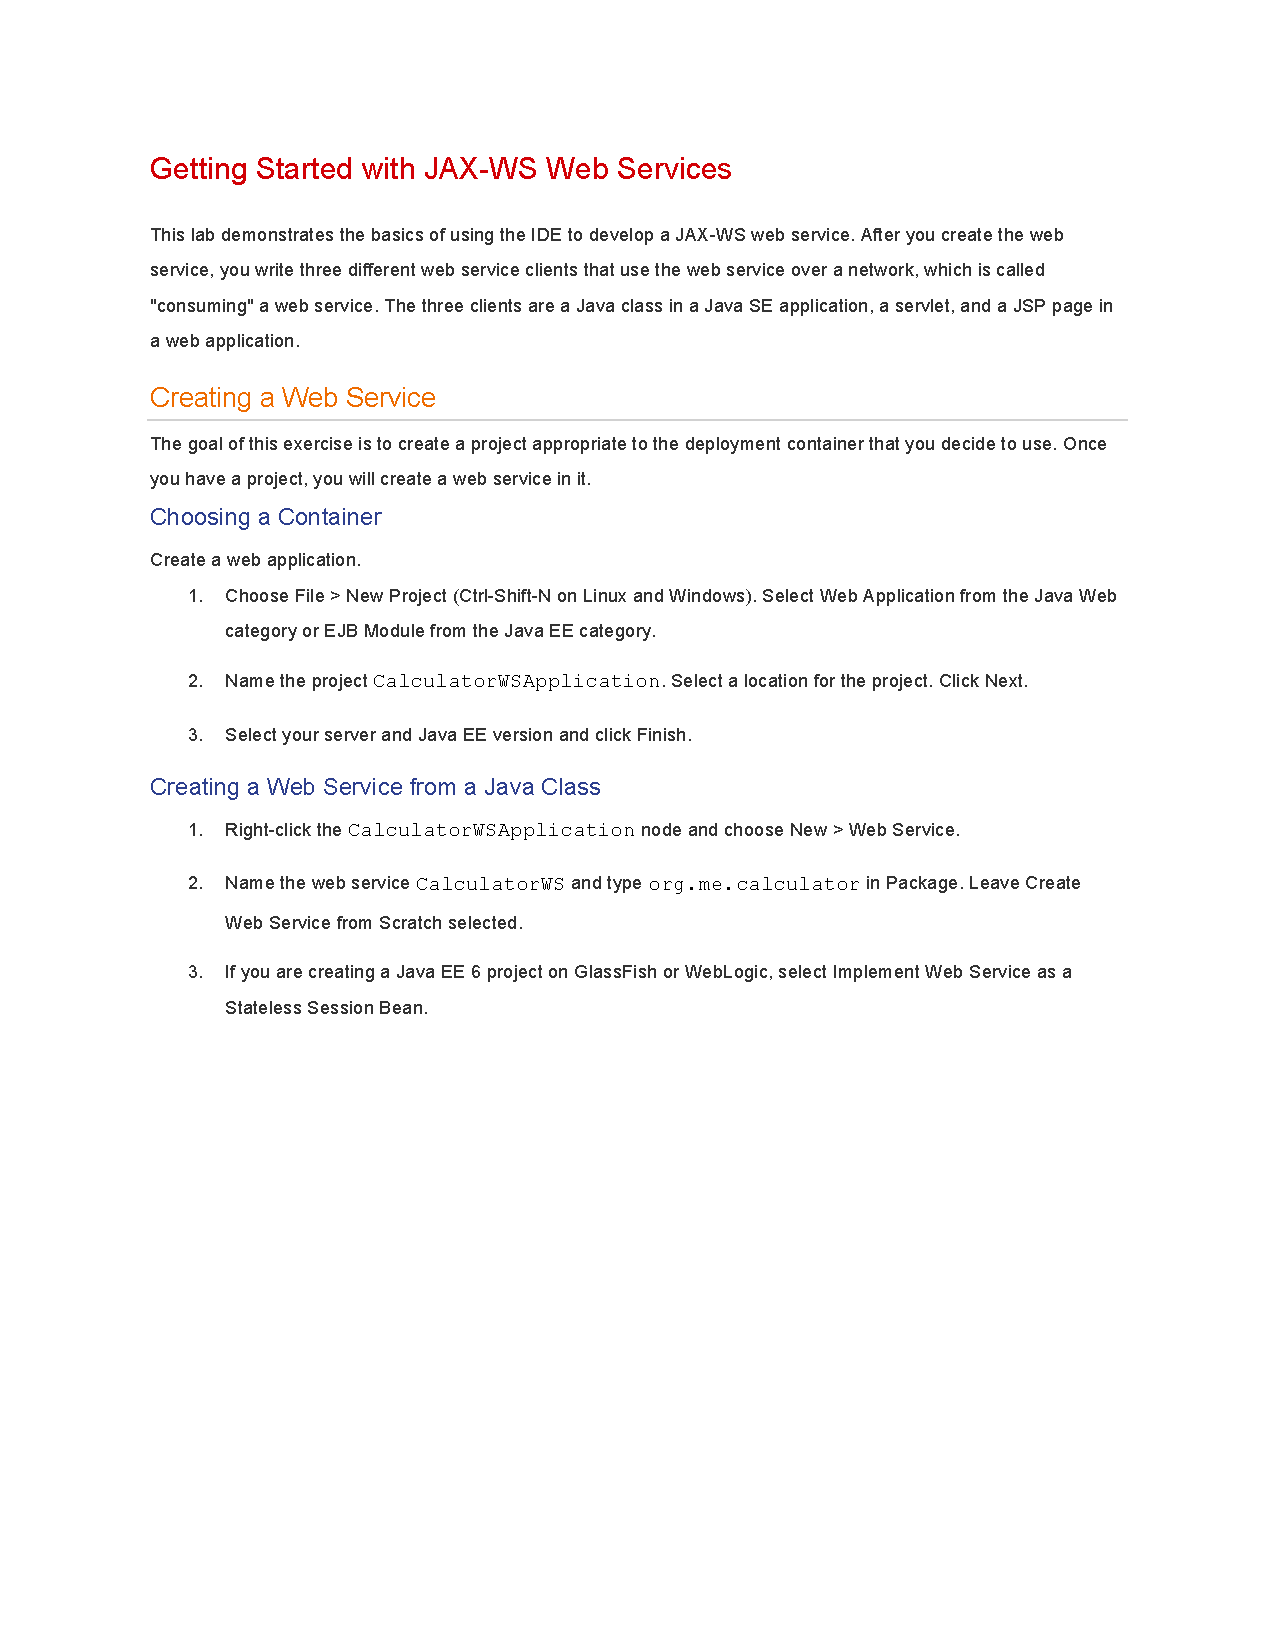
\includepdf[pages={-}]{NetbeansJava.pdf}

\section{JAVA Questions}
\label{JavaQuestionsTrueFalse}
\begin{enumerate}
\item Assembly language is the language that uses mnemonics for its instructions.
\item The arithmetic operations are performed inside CPU and, if an error is found, it outputs the logical errors.
\item A Java compiler is a program that translates a Java program into bytecode.
\item Bytecode is the machine language of the JVM.
\item The CPU stands for command performing unit.
\item RAM stands for readily available memory.
\item A program written in a high-level programming language is called a source program.
\item The operating system is the first program loaded into the computer when the power is turned on.
\item The first step in the problem-solving process is to analyze the problem.
\item An identifier can be any sequence of digits and letters.
\item In Java, there is no difference between a reserved word and a predefined identifier.
\item A Java identifier can start with a digit.
\item The operands of the modulus operator must be integers.
\item If the value of a is 4 and the value of b is 3, the n after the statement a=b; the value of b is still 3.
\item In an output statement, the newline character may be a part of the string.
\item The following is a legal Java program:
\begin{lstlisting}
public class JavaProgram {
public static void main(String[] args) {
	}
}
\end{lstlisting}
\item In a mixed expression, all operands are converted to floating-point numbers.
\item Suppose x = 5. After the statement y = x++; executes, y is 5 and x is 6.
\item Suppose a = 5. After the statement ++a; executes, the value of a is still 5 because the value of the expression is not saved in another variable.
\item A variable declared using a class is called an object.
\item In the statement x 1⁄4 console.nextInt() ;, x must be a variable.
\item You generate the newline character by pressing Enter (return) on the keyboard.
\item The methods printf and format are used to format a decimal number to a specific number of decimal places.
\item The result of a logical expression cannot be assigned to an int variable. 
\item In a one-way selection, if a semicolon is placed after the expression in an if statement, the expression in the if statement is always true. 
\item Every if statement must have a corresponding else.
\item The expression:
\begin{lstlisting}
(ch >= 'A' && ch <= 'Z')
\end{lstlisting}
evaluates to false if either ch < 'A' or ch >= 'Z'.
\item Suppose the input is 5. (Assume that all variables are properly declared.) The output of the code:
\begin{lstlisting}
num = console.nextInt(); 
if (num > 5)
    System.out.println(num);
num = 0;
else
	System.out.println("Num is zero");
\end{lstlisting}
is: Num is zero.
\item The expression in a switch statement should evaluate to a value of any primitive data type.
\item The expression !(x > 0) is true only if x is a negative number. 
\item In Java, both ! and != are logical operators.
\item The order in which statements execute in a program is called the flow of control.
\item In a counter-controlled while loop, it is not necessary to initialize the loop control variable.
\item It is possible that the body of a while loop might not execute at all.
\item In an infinite while loop, the loop condition is initially false, but after the first iteration, it is always true.
\item The while loop:
\begin{lstlisting}
j = 0;
while (j <= 10) j++;
\end{lstlisting}
terminates when j > 10.
\item A sentinel-controlled while loop is an event-controlled while loop whose termination depends on a special value.
\item A loop is a control structure that causes certain statements to execute over and over.
\item To read data from a file of an unspecified length, an EOF-controlled loop is a good choice.
\item When a while loop terminates, the control first goes back to the statement just before the while statement, and then the control goes to the statement immediately following the while loop.
\item Every window has a width and height.
\item In Java, JFrame is a class.
\item To display the window, you need not invoke a method such as setVisible.
\item In Java, the reserved word extends allows you to create a new class from an existing one.
\item The window you see displayed on your screen is a class.
\item Labels are used to display the output of a program.
\item Every GUI component you need has to be created and added to a container.
\item In Java, implements is a keyword.
\item Clicking a button is an example of an action event.
\item In a problem statement, every verb is a possible class.
\item In a problem statement, every noun is a possible method.
\item To use an object, you must know how it is implemented.
\item To use a predefined method of a class contained in the package java.lang in a program, you only need to know what the name of the method is and how to use it.
\item A value-returning method returns only one value via the return statement.
\item Parameters allow you to use different values each time the method is called.
\item When a return statement executes in a user-defined method, the method immediately exits.
\item A value-returning method returns only integer values.
\item If a Java method does not use parameters, parentheses around the empty parameter list are still needed.
\item In Java, the names of the corresponding formal and actual parameters must be the same.
\item In Java, method definitions can be nested; that is, the definition of one method can be enclosed in the body of another method.
\item The instance variables of a class must be of the same type.
\item The methods of a class must be public.
\item A class can have more than one constructor.
\item A constructor can return a value of the int type.
\item An accessor method of a class accesses and modifies the data members of the class.
\item A double type is an example of a primitive data type.
\item A one-dimensional array is an example of a structured data type.
\item Arrays can be passed as parameters to a method.
\item A method can return a value of the type array.
\item The size of an array is determined at compile time.
\item Given the declaration:
\begin{lstlisting}
int[] list = new int[10];
\end{lstlisting}
the statement:
\begin{lstlisting}
list[5] = list[3] + list[2];
\end{lstlisting}
updates the content of the fifth element of the array list.
\item If an array index goes out of bounds, the program terminates in an error.
\item The constructor of a subclass specifies a call to the constructor of the superclass in the heading of the constructor’s definition.
\item The constructor of a subclass specifies a call to the constructor of the superclass using the name of the class.
\item A subclass must define a constructor.
\item In Java, polymorphism is implemented using late binding.
\item The block finally is always executed.
\item Division by zero is a checked exception.
\item File not found is an unchecked exception.
\item Exceptions are thrown either in a try block in a method or from a method called directly or indirectly from a try block.
\item The order in which catch blocks are listed is not important.
\item An exception can be caught either in the method where it occurred or in any one of the methods that led to the invocation of this method.
\item One way to handle an exception is to print an error message and exit the program.
\item All excAepptioansgmoust bPe rDepFortedEtonahvoaidncocmepilration errors.
\item An event handler is a method.
\item A GUI component can generate only one type of event.
\item An applet’s width and height are specified in the HTML file.
\item In Java, JApplet is a class.
\item To display an applet, you do not need to invoke a method, such as setVisible().
\item You must include an exit button in all Java applets.
\item When an applet is loaded, the method start is invoked before the method init.
\item Check boxes are used to display the output of a program.
\item A radio button always has a label.
\item You use JList to create a combo box.
\item JTextField can be used to output multiple lines of text.
\item Every recursive definition must have one or more base cases.
\item Every recursive method must have one or more base cases.
\item The general case stops the recursion.
\item In the general case, the solution to the problem is obtained directly.
\item A recursive method always returns a value.
\end{enumerate}


\section{Answers to JAVA Questions}
This section presents answers to questions presented in \ref{JavaQuestionsTrueFalse} in page \pageref{JavaQuestionsTrueFalse}
\begin{enumerate}
\item True
\item False
\item True
\item True
\item False
\item False
\item True
\item True
\item True
\item False
\item False
\item False
\item False
\item True
\item True
\item True
\item False
\item True
\item False
\item False
\item True
\item True
\item True
\item True
\item False
\item False
\item False
\item False
\item False
\item False
\item False
\item True
\item False
\item True
\item False
\item True
\item True
\item True
\item True
\item False
\item True
\item True
\item True
\item True
\item False
\item False
\item True
\item True
\item True
\item False
\item False
\item False
\item True
\item True
\item True
\item True
\item False
\item True
\item False
\item False
\item False
\item False
\item True
\item False
\item False
\item True
\item True
\item True
\item True
\item False
\item False
\item True
\item False
\item False
\item False
\item True
\item True
\item False
\item False
\item True
\item False
\item True
\item True
\item False
\item True
\item False
\item True
\item True
\item True
\item False
\item False
\item False
\item True
\item False
\item False
\item True
\item True
\item False
\item False
\item False
\end{enumerate}


\end{document}